%
% File acl2021.tex
%
%% Based on the style files for EMNLP 2020, which were
%% Based on the style files for ACL 2020, which were
%% Based on the style files for ACL 2018, NAACL 2018/19, which were
%% Based on the style files for ACL-2015, with some improvements
%%  taken from the NAACL-2016 style
%% Based on the style files for ACL-2014, which were, in turn,
%% based on ACL-2013, ACL-2012, ACL-2011, ACL-2010, ACL-IJCNLP-2009,
%% EACL-2009, IJCNLP-2008...
%% Based on the style files for EACL 2006 by 
%%e.agirre@ehu.es or Sergi.Balari@uab.es
%% and that of ACL 08 by Joakim Nivre and Noah Smith

\documentclass[11pt,a4paper]{article}
\usepackage[hyperref]{acl2021}
\usepackage{times}
\usepackage{amsmath}
\usepackage{latexsym}
\usepackage{graphicx}

\renewcommand{\UrlFont}{\ttfamily\small}
\graphicspath{ {./images/} }

% This is not strictly necessary, and may be commented out,
% but it will improve the layout of the manuscript,
% and will typically save some space.
\usepackage{microtype}
\usepackage{booktabs}
\usepackage{float}


\aclfinalcopy % Uncomment this line for the final submission
%\def\aclpaperid{***} %  Enter the acl Paper ID here

%\setlength\titlebox{5cm}
% You can expand the titlebox if you need extra space
% to show all the authors. Please do not make the titlebox
% smaller than 5cm (the original size); we will check this
% in the camera-ready version and ask you to change it back.

\newcommand\BibTeX{B\textsc{ib}\TeX}

\title{Homework 2: Aspect-Based Sentiment Analysis}

\author{Michele Conti \\
	\texttt{conti.1599133@studenti.uniroma1.it}\\}

\date{}

\begin{document}
	\maketitle
	\section{Introduction}
	Aspect-based sentiment analysis (ABSA) tackles the problem of finding both
	aspects in a given sentence, and the polarities associated with those aspects.
	For example, given the sentence "I love their pasta but I hate their Ananas
	Pizza", the task is to first extract the two aspects "pasta" and "Ananas Pizza",
	and to then to predict their associated polarities, in this case respectively
	"positive" and "negative".
	
	In this paper, I propose an end-to-end approach to attack this task, exploiting
	the combination of both context-independent (GloVe) and context-dependent (BERT)
	word embeddings, multihead attention layers, and the use of a BiLSTM layer,
	reaching satisfying results on the provided development dataset (macro f1 score
	of 0.544 on the Restaurants + Laptops development set).
	
	\section{Problem formulation}
	All the model variations proposed in this paper tackle the ABSA problem in an
	end-to-end fashion, meaning that both tasks (i.e., aspect sentiment extraction
	and aspect sentiment polarity evaluation) are solved simultaneously. To achieve
	this, the two-sided problem has been formulated as a sequence labeling task. 
	
	To that end, this is the general pipeline followed: during the preprocessing,
	each token of each sentence is tagged using either an IOB (i.e., Inside,
	Outside, Beginning) or a BIOES (i.e., Beginning, Inside, Outside, Ending,
	Single) tagging schema, used on top of the four polarities appearing in the
	datasets (example of the two tagging schemas in figure \ref{fig:IOB_BIOES}).
	Depending on the adopted tagging schema, the model is then trained to extract
	the right label from a set of either  $4 \cdot 2 + 1 = 9$ (for IOB) or $4 \cdot
	4 + 1 = 17$ (for BIOES) possible classes. Finally, the model output is
	translated back into its original form, where the tokens classified as "O" are
	not considered and the aspect terms are merged together according to their tags
	(e.g., \{"Ananas" = B-negative, "Pizza" = I-negative\} $\to$ \{"Ananas Pizza" =
	negative\}).
	
	\section{Models}
	In this section, I will present all the modules that compose the proposed final
	model, starting by introducing the structure of the baseline network. Then, at
	each step, I will introduce the very next module used, describing its main
	functionalities and analyzing the boost in terms of performance when added to
	the network.
	
	To evaluate the performance of the following models, I will use their macro f1
	score on the combined task of aspect term extraction and evaluation.
	
	Moreover, IOB has been selected as the preferred tagging schema, and all the
	following model performances are computed using that. Finally, all models have
	been trained using AdamW as optimizer.
	
	\subsection{M0: Baseline}
	The first model used to solve the ABSA task is a very simple network, composed
	by an embedding layer to encode the tokens of the input sentences, followed by a
	one-on-one linear layer (i.e., input features equal to output features), two
	stacked BiLSTM layers and a prediction block, composed by a linear layer and a
	softmax activation (network architecture in figure \ref{fig:M0_architecture}).
	Additionally, I replaced the randomly initialized word embeddings in the
	embedding layer with the pre-trained word vectors of GloVe
	\citep{pennington2014glove}.
	
	In this first model variation, no contextual information is considered in the
	embedding phase, since the word embeddings provided by GloVe, being
	context-free, will produce the same vector representation regardless of the
	context. Nevertheless, the BiLSTM layers partially make up for this, encoding
	both the left-to-right and the right-to-left context for each word of a
	sentence.
	
	This very simple architecture (let's call it M0) is still able to achieve
	decent results in terms of f1 score, reaching a maximum of 0.381 in terms of
	macro f1 score (see figures \ref{fig:M0_loss}, \ref{fig:M0_extr},
	\ref{fig:M0_eval} respectively for the loss plots, f1 extraction and f1
	extraction + evaluation plots on the train. and dev. datasets).
	
	\subsection{M1: BERT Embedder}
	To add contextual information to my model, I decided to use BERT (Bidirectional
	Encoder Representations Transformers) \citep{devlin2018bert}. BERT is a language
	representation model, which uses bidirectional transformers to pre-train on a
	very large corpus over different pre-training tasks. Then, the pre-trained BERT
	model can be fine-tuned to be used on other tasks. In my case, I decided to use
	BERT as an embeding layer, as suggested in \citep{li2019exploiting}. Differently
	from the traditional GloVe based embedding layer, which, as I already said,
	provide only context-independent representation for each token, using BERT as an
	embedding layer does provide context-dependant information about each token in a
	sentence.
	
	To get the most out of BERT, I followed one of the approaches proposed in
	\citep{acs2021subword} as pooling strategy. In particular, the approach can be
	summarized in two steps: first, the BERT embeddings for the subwords of each
	token are computed. This is achieved by averaging the last 3 hidden layers of
	BERT. Then, the weighted average of the subwords embeddings are computed, based
	on the BPE length of each token.
	
	This process can be carried out in two ways: keeping the BERT parameters
	freezed, or keeping them free and finetuning them during the training process.
	These two possible choices are the basis of a trade off between two possible
	scenarios: on the one hand, keeping the BERT weights freezed, we have a much
	easier time when training our model, in terms of both training time, and
	flexibility in the choice of the hyperparameters. On the other, learning also
	the parameters for the BERT model gives the chance to, potentially, achieve much
	better results.
	
	Once the BERT embeddings have been computed, similarly to the GloVe embeddings,
	they are too passed into a linear layer with a ReLU activation, and subsequently
	concatenated with the GloVe pretrained embeddings. The rest of the network is
	the same. Adding context-dependent information with BERT and keeping its
	parameters freezed (let's call this model M1), the model reaches 0.466 macro f1
	score on the dev set.
	
	\subsection{M2: Finetuning BERT}
	As already discussed, there is a big trade-off between training feasibility and
	performances. Obviously, exploiting the general representation given by BERT for
	such a fine-grained task as aspect based sentiment analysis is far from ideal,
	and therefore it just makes sense to fine-tune the BERT parameters. In order to
	do so, I noticed that the value for the optimizer learning rate really made a
	difference when fine-tuning the BERT embedder. Once a good value for that was
	found, I was able to reach 0.497 macro f1 score on the development set, just by
	unblocking the BERT parameters.
	
	\subsection{M3: Self-Attention}
	Self-attention is an attention mechanism relating different positions
	of a single sequence in order to compute a representation of the same sequence.
	It has been made popular by \citep{vaswani2017attention}, and, intuitively, it
	makes it possible for the network to focus on relevant parts of a sentence. The
	attention scores are computed as follows:
	
	\begin{equation}
	\mathrm{Attention}(Q, K, V) = \mathrm{softmax}(\frac{QK^T}{\sqrt{d_k}})V
	\end{equation}
	
	To attend different parts of a sentence, multiple attention heads can be
	computed and then concatenated. The resulting vector can be then linearly
	transformed into the expected dimension. This process is known as Multi-head
	Attention.
	
	For my use case, I used Multi-head Attention as a feature extractor on both the
	GloVe embeddings and on the BERT embeddings, respectively using 12 and 24 heads.
	Then, as in the previous versions, I concatenated the two resulting embeddings,
	and passed the result to the stacked BiLSTM layers and to the prediction block.
	
	This was the trick that made me achieve the best results, achieving 0.544 macro
	f1 score on the development set. Therefore, this is the final proposed model for
	this homework (see figure \ref{fig:M3_architecture} for the model architecture,
	figures \ref{fig:M3_loss}, \ref{fig:M3_extr}, \ref{fig:M3_eval} respectively for
	the loss plots, f1 extraction and f1 extraction + evaluation plots on the train.
	and dev. datasets).
	
	\section{Honorable mentions}
	In this section I'll briefly talk about two techniques that I applied, and for
	which I had good expectations, but which, unfortunately, didn't translate
	directly into better performances.
	
	\subsection{M4: Conditional Random Field}
	Conditional Random Fields \citep{lafferty2001conditional} are very often used
	with success in sequence labeling tasks such as named entity recognition, as
	they model the likelihood of a given sequence, implementing dependencies between
	the predictions.  For this reason, it seemed like a natural choice to adopt this
	approach in my use case. Unfortunately, this wasn't the case, as, using CRF, the
	model performance has dropped to 0.493. I suspect that the reason behind it is
	that the embeddings computed with BERT provide enough information for a linear
	layer to work just better. In fact, removing the BERT embeddings and relying
	only on context-free embeddings given by GloVe, the CRF actually makes a
	difference, increasing the performances of the baseline model to 0.391 (from
	0.381).
	
	\subsection{M5: POS embeddings}
	In theory, part-of-speech tags should be an important tool, specifically in the
	aspect term extraction part. In fact, most of the aspect terms are represented
	by nouns, and therefore identifying the part of speech should at least work as a
	first selection, to rule out words that are very unlikely to be aspect terms. In
	practice, this didn't turn out to be true. I guess that there are several
	reasons why this is the case. First of all, the dataset doesn't provide a gold
	label for the POS tags of the tokens, and therefore, we must produce our own POS
	tags using a pretrained model. This means that we are injecting in our data a
	new potential source of errors, since the non-manually tagged data could be
	wrong in the first place.
	
	Additionally, the aspect extraction task isn't that hard, in fact all models,
	even the baseline one, behave quite well on that task (see figure
	\ref{fig:comparative_f1_extr}).
	
	For these reasons, embedding the POS tags and concatenating that to the other
	word representations made the performances drop to 0.509.
	
	\section{Conclusion}
	In this paper I have analyzed the performance of various models. In the end, I think I have reached satisfactory results. Moreover, I
	think that the use of an end-to-end model for this task can be very beneficial
	for its simplicity, as it really needs very basic preprocessing on the text to
	be set up, and the output can be postprocessed trivially.
	
	An ablation study is proposed in the final section. Specifically, see table \ref{tab:hyperparams} for the hyperparameters of the proposed model, table 
	\ref{tab:ab_ablation} for the performances of all the models,
	table \ref{tab:ab_iob_bioes} for the comparison between the proposed model using
	IOB vs the BIOES, figures \ref{fig:comparative_f1_extr} and
	\ref{fig:comparative_f1_eval} for the f1 score in terms
	of extraction and extraction + evaluation for all the models, and figures \ref{fig:cm_M0} and \ref{fig:cm_M3} for the confusion matrices of the baseline and of the proposed model.
	
	\section{Extra}
	In this section I will talk about the additional optional task proposed, namely the combination of aspect category identification and aspect category polarity classification. For example, given the sentence "Prices are higher to dine in and their chicken tikka marsala is quite good", the task is to identify the two categories "food" and "price", and to then predict their associated polarities, in this case respectively "positive" and "negative".
	
	The model proposed for this task directly inherits from the model used to tackle the previous tasks, and the only modification is made on the classification head, as this can no more be considered a sequence labeling task. Instead, the model has to make five independet predictions for a given sentence, one for each category ("anecdotes/miscellaneous", "price", "food", "ambience", "service"). Each prediction will span across 5 possible classes, which are the 4 traditional polarities ("positive", "negative", "neutral", "conflict") and one additional non-polarity "O", representing the fact that the input sentence does not have the selected category between the its aspect categories.
	
	This way, this problem too can be approached in an end-to-end fashion, without modifying too much the initial structure proposed. Indeed, using this approach, I am able to reach satisfactory results also in this additional task, reaching 0.576 macro f1 score on the task of category extraction + polarity evaluation on the development set (that, in this case, is represented by the only Restaurants dataset).
	
	One final consideration can be made on this additional task. I think that the the connection between the two tasks could be exploited: for instance, an attempt could be made to use the predictions of the first model as input of the second model.
	
	\clearpage
	\section{Figures and tables}
	All figures and tables have been intentionally placed at the end of the
	document, in this section, so that they don't affect the maximum limit of three
	pages for the text.
	
	\begin{table}[H]
		\centering
		\begin{tabular}{@{}lcc@{}}
			\toprule
			\textbf{Sentiment} & Train & Dev \\ \midrule
			positive           & 2605  & 546 \\
			negative           & 1364  & 307 \\
			neutral            & 877   & 216 \\
			conflict           & 111   & 25  \\ \bottomrule
		\end{tabular}
		\caption{Polarities support for targets (task A+B) in the training and
			development set (i.e., Restaurants + Laptops).}
		\label{tab:ab_polarities_support}
	\end{table}

	\begin{table}[H]
		\centering
		\begin{tabular}{@{}ll@{}}
			\toprule
			\textbf{Hyperparameters}                  & Value \\ \midrule
			Tagging schema                            & IOB   \\
			Vocabularies min. freq.                   & 2     \\
			Batch size                                & 16    \\
			Optimizer                                 & AdamW \\
			Learning rate                             & 2e-5  \\
			Weight decay                              & 0.0   \\
			GloVe embeddings size                     & 300   \\
			BERT embeddings                           & 768   \\
			BiLSTM layers                             & 2     \\
			BiLSTM hidden dim.                        & 300   \\
			Activation functions                      & ReLU  \\ \bottomrule
		\end{tabular}
		\caption{Hyperparameters for the proposed model.}
		\label{tab:hyperparams}
	\end{table}
	
	\begin{table}[H]
		\centering
		\begin{tabular}{@{}lcc@{}}
			\toprule
			\textbf{Category}         & Train     & Dev \\ \midrule
			anecdotes/miscellaneous   & 941       & 191     \\
			price                     & 268       & 53      \\
			food                      & 1008      & 224     \\
			ambience                  & 355       & 76      \\
			service                   & 478       & 119     \\ \bottomrule
		\end{tabular}
		\caption{Categories support (task C+D) in the training and development set
			(i.e., Restaurants).}
		\label{tab:cd_categories_support}
	\end{table}
	
	\begin{table}[H]
		\centering
		\begin{tabular}{@{}lcc@{}}
			\toprule
			\textbf{Sentiment} & Train & Dev \\ \midrule
			positive           & 1803  & 376 \\
			negative           & 672   & 167 \\
			neutral            & 411   & 89  \\
			conflict           & 164   & 31  \\ \bottomrule
		\end{tabular}
		\caption{Polarities support for categories (task C+D) in the training and
			development set (i.e., Restaurants).}
		\label{tab:cd_polarities_support}
	\end{table}
	
	
	\begin{table}[H]
		\centering
		\begin{tabular}{@{}lcc@{}}
			\toprule
			\textbf{Model}         & F1 Extr.       & F1 Eval.       \\ \midrule
			M0 = Baseline          & 0.715          & 0.381          \\
			M1 = M0 + BERT$_{freeze}$         & 0.805          & 0.466          \\
			M2 = M0 + BERT$_{finetune}$        & 0.801          & 0.497          \\
			\textbf{M3 = M2 + ATT} & \textbf{0.820} & \textbf{0.544} \\
			\midrule
			M4 = M3 + CRF          & 0.813          & 0.493          \\
			M5 = M3 + POS          & 0.798          & 0.509          \\ \bottomrule
		\end{tabular}
		\caption{Task A+B: Models variations top performance on development set
			(Restaurants + Laptops). For each variation, it has been selected the model with
			the highest f1 evaluation score on the validation set. \\ The baseline model
			(M0) is the one discussed in section (?). With "BERT" I refer to the BERT
			Embedder introduced in section (?) (BERT$_{freeze}$ means that the BERT Embedder
			is based on a pretrained version of the BERT model, and that there is no
			finetuning involved during the training. Instead, BERT$_{finetune}$ means that
			the BERT model is initially loaded from a pretrained version, but it is also
			finetuned during training). With "ATT" I refer to a multihead self attention
			layer, as discussed in section (?). With "CRF" I refer to Conditional Random
			Field, as discussed in section (?). With "POS", I refer to the use of an
			embedding layer for the part-of-speech tags of the tokens of each sentence, as
			discussed in section (?).}
		\label{tab:ab_ablation}
	\end{table}
	
	\begin{table}[H]
		\centering
		\begin{tabular}{@{}lcc@{}}
			\toprule
			\textbf{Model}                        & F1 Extr.       & F1 Eval.       \\
			\midrule
			\textbf{M3$_{\mathbf{IOB}}$} & \textbf{0.820} & \textbf{0.544} \\
			M3$_{\mathrm{BIOES}}$                         & 0.812          & 0.490       
			\\ \bottomrule
		\end{tabular}
		\caption{Task A+B: Proposed model top performance comparison using two tagging
			schemas: IOB (i.e., Inside-Outside-Beginning), and BIOES (i.e., beginning,
			inside, outside, end, single).}
		\label{tab:ab_iob_bioes}
	\end{table}
	
	\begin{figure}[H]
		\centering
		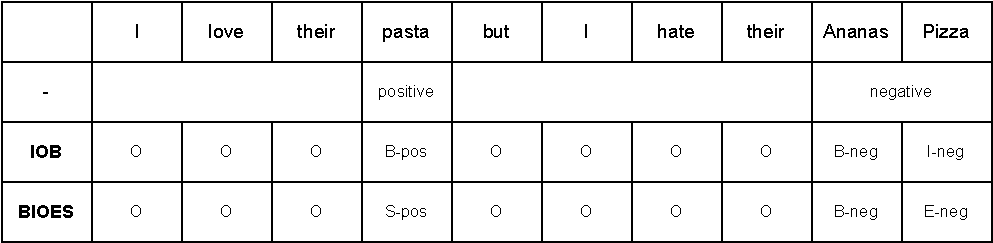
\includegraphics[width=1\columnwidth]{IOB_BIOES_example.pdf}
		\caption{IOB and BIOES tagging schemas example.}
		\label{fig:IOB_BIOES}
	\end{figure}
	
	\begin{figure}[H]
		\centering
		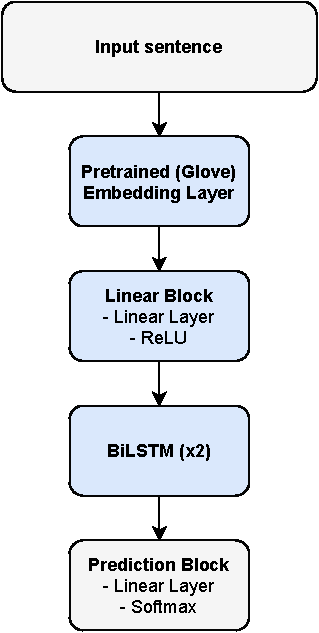
\includegraphics[width=0.7\columnwidth]{M0_diagram.pdf}
		\caption{Baseline model (M0) architecture.}
		\label{fig:M0_architecture}
	\end{figure}
	
	
	\begin{figure}[H]
		\centering
		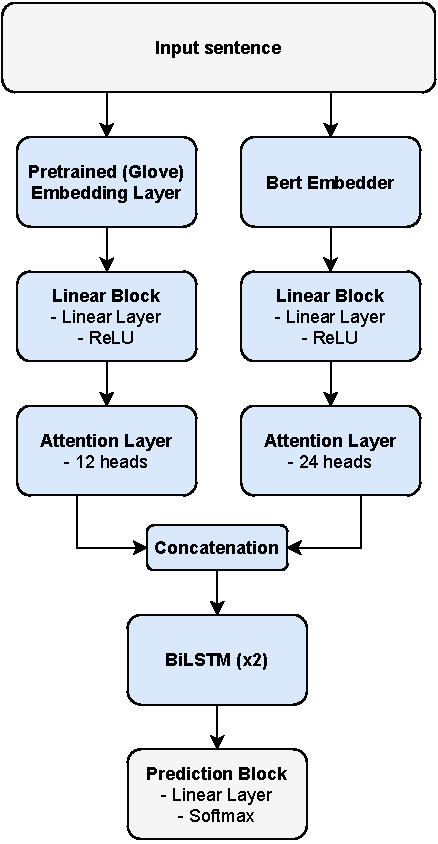
\includegraphics[width=0.9\columnwidth]{M3_diagram.pdf}
		\caption{Final model (M3) architecture.}
		\label{fig:M3_architecture}
	\end{figure}
	
	
	
	\begin{figure}[H]
		\centering
		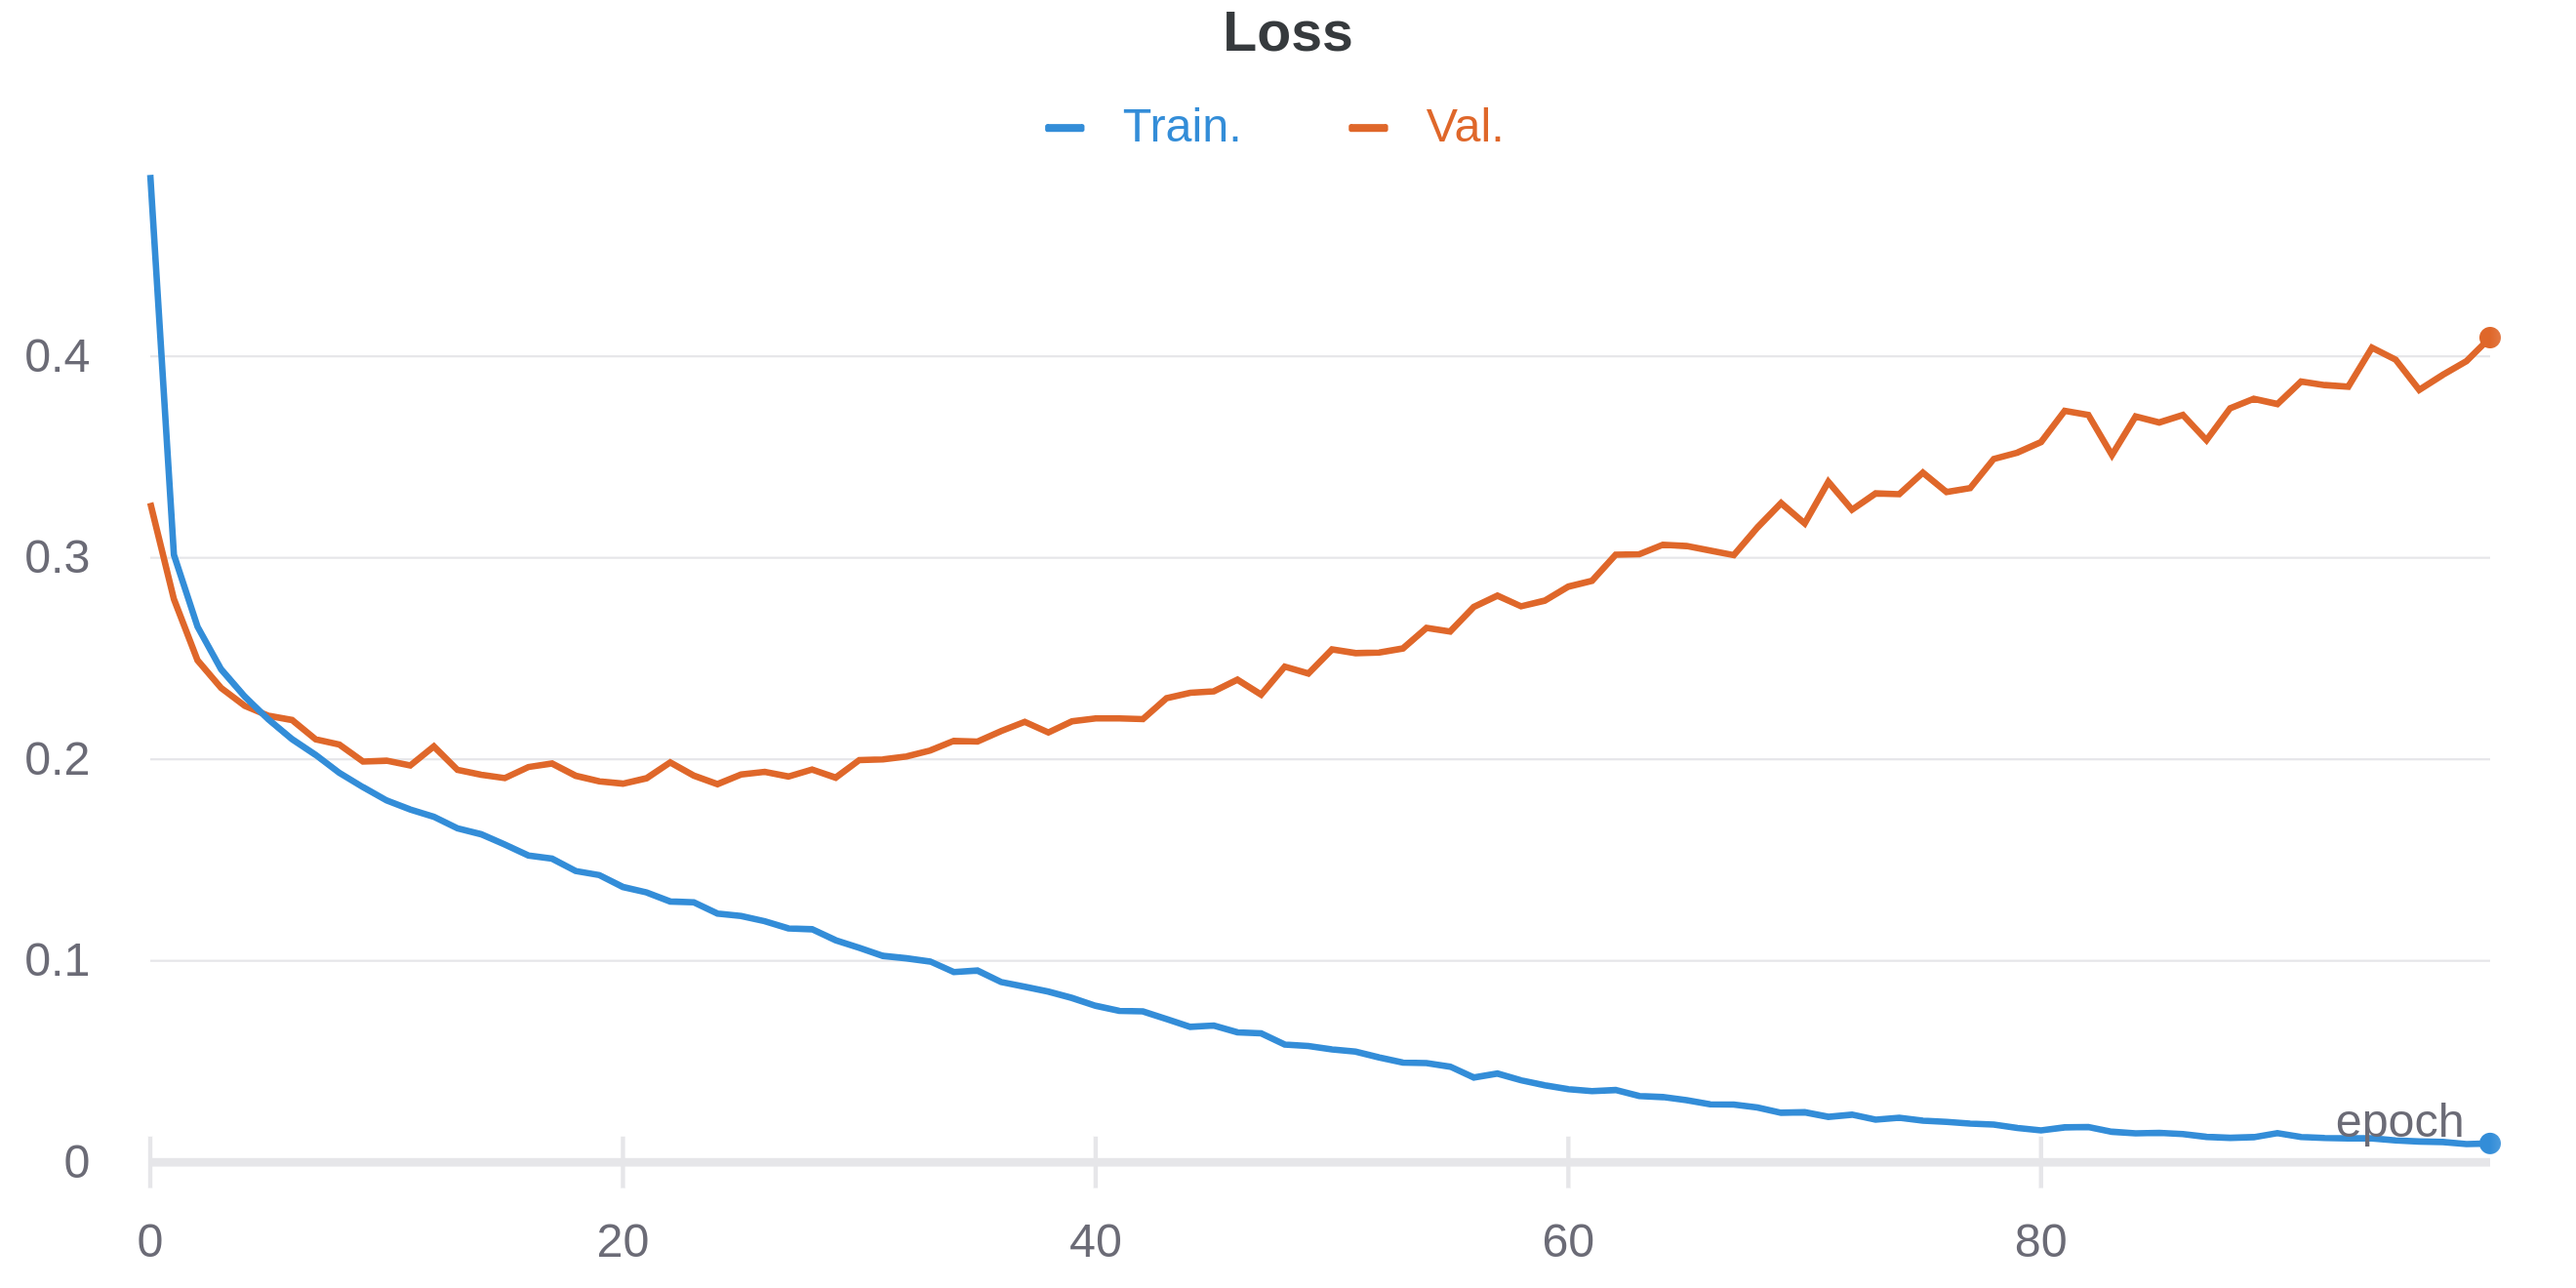
\includegraphics[width=1\columnwidth]{M0_ab_loss.png}
		\caption{Task A+B: Baseline (M0) loss on the training and development set.}
		\label{fig:M0_loss}
	\end{figure}
	
	\begin{figure}[H]
		\centering
		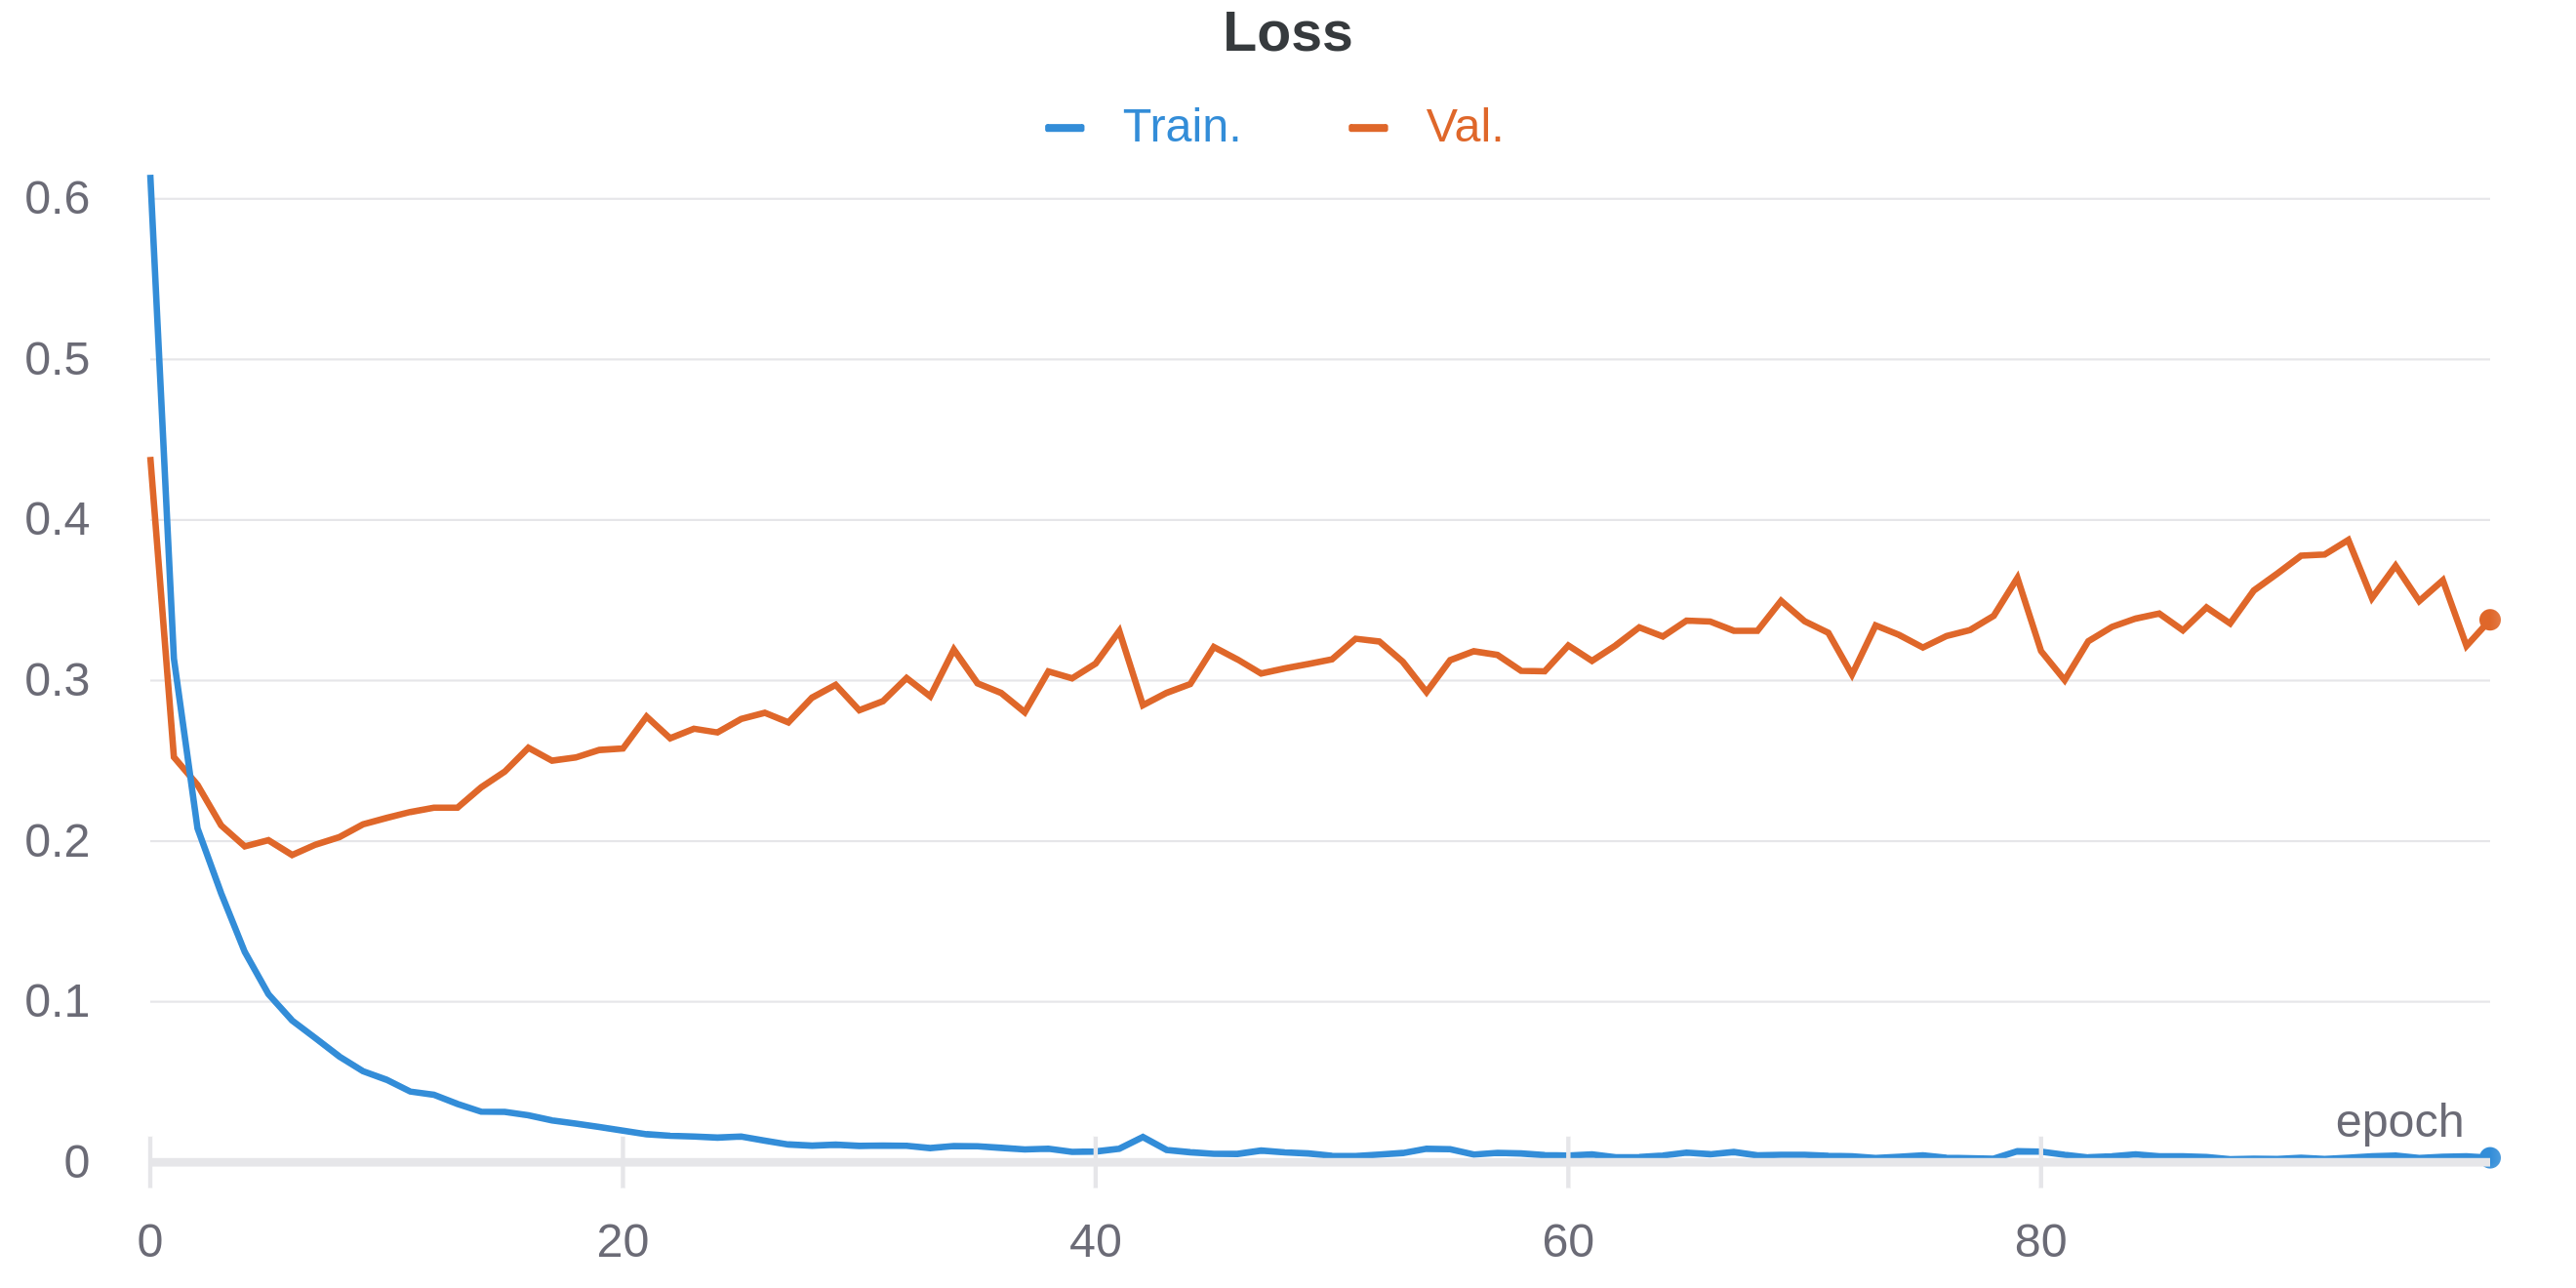
\includegraphics[width=1\columnwidth]{M3_ab_loss.png}
		\caption{Task A+B: Final model (M3) loss on the training and development set.}
		\label{fig:M3_loss}
	\end{figure}
	
	\begin{figure}[H]
		\centering
		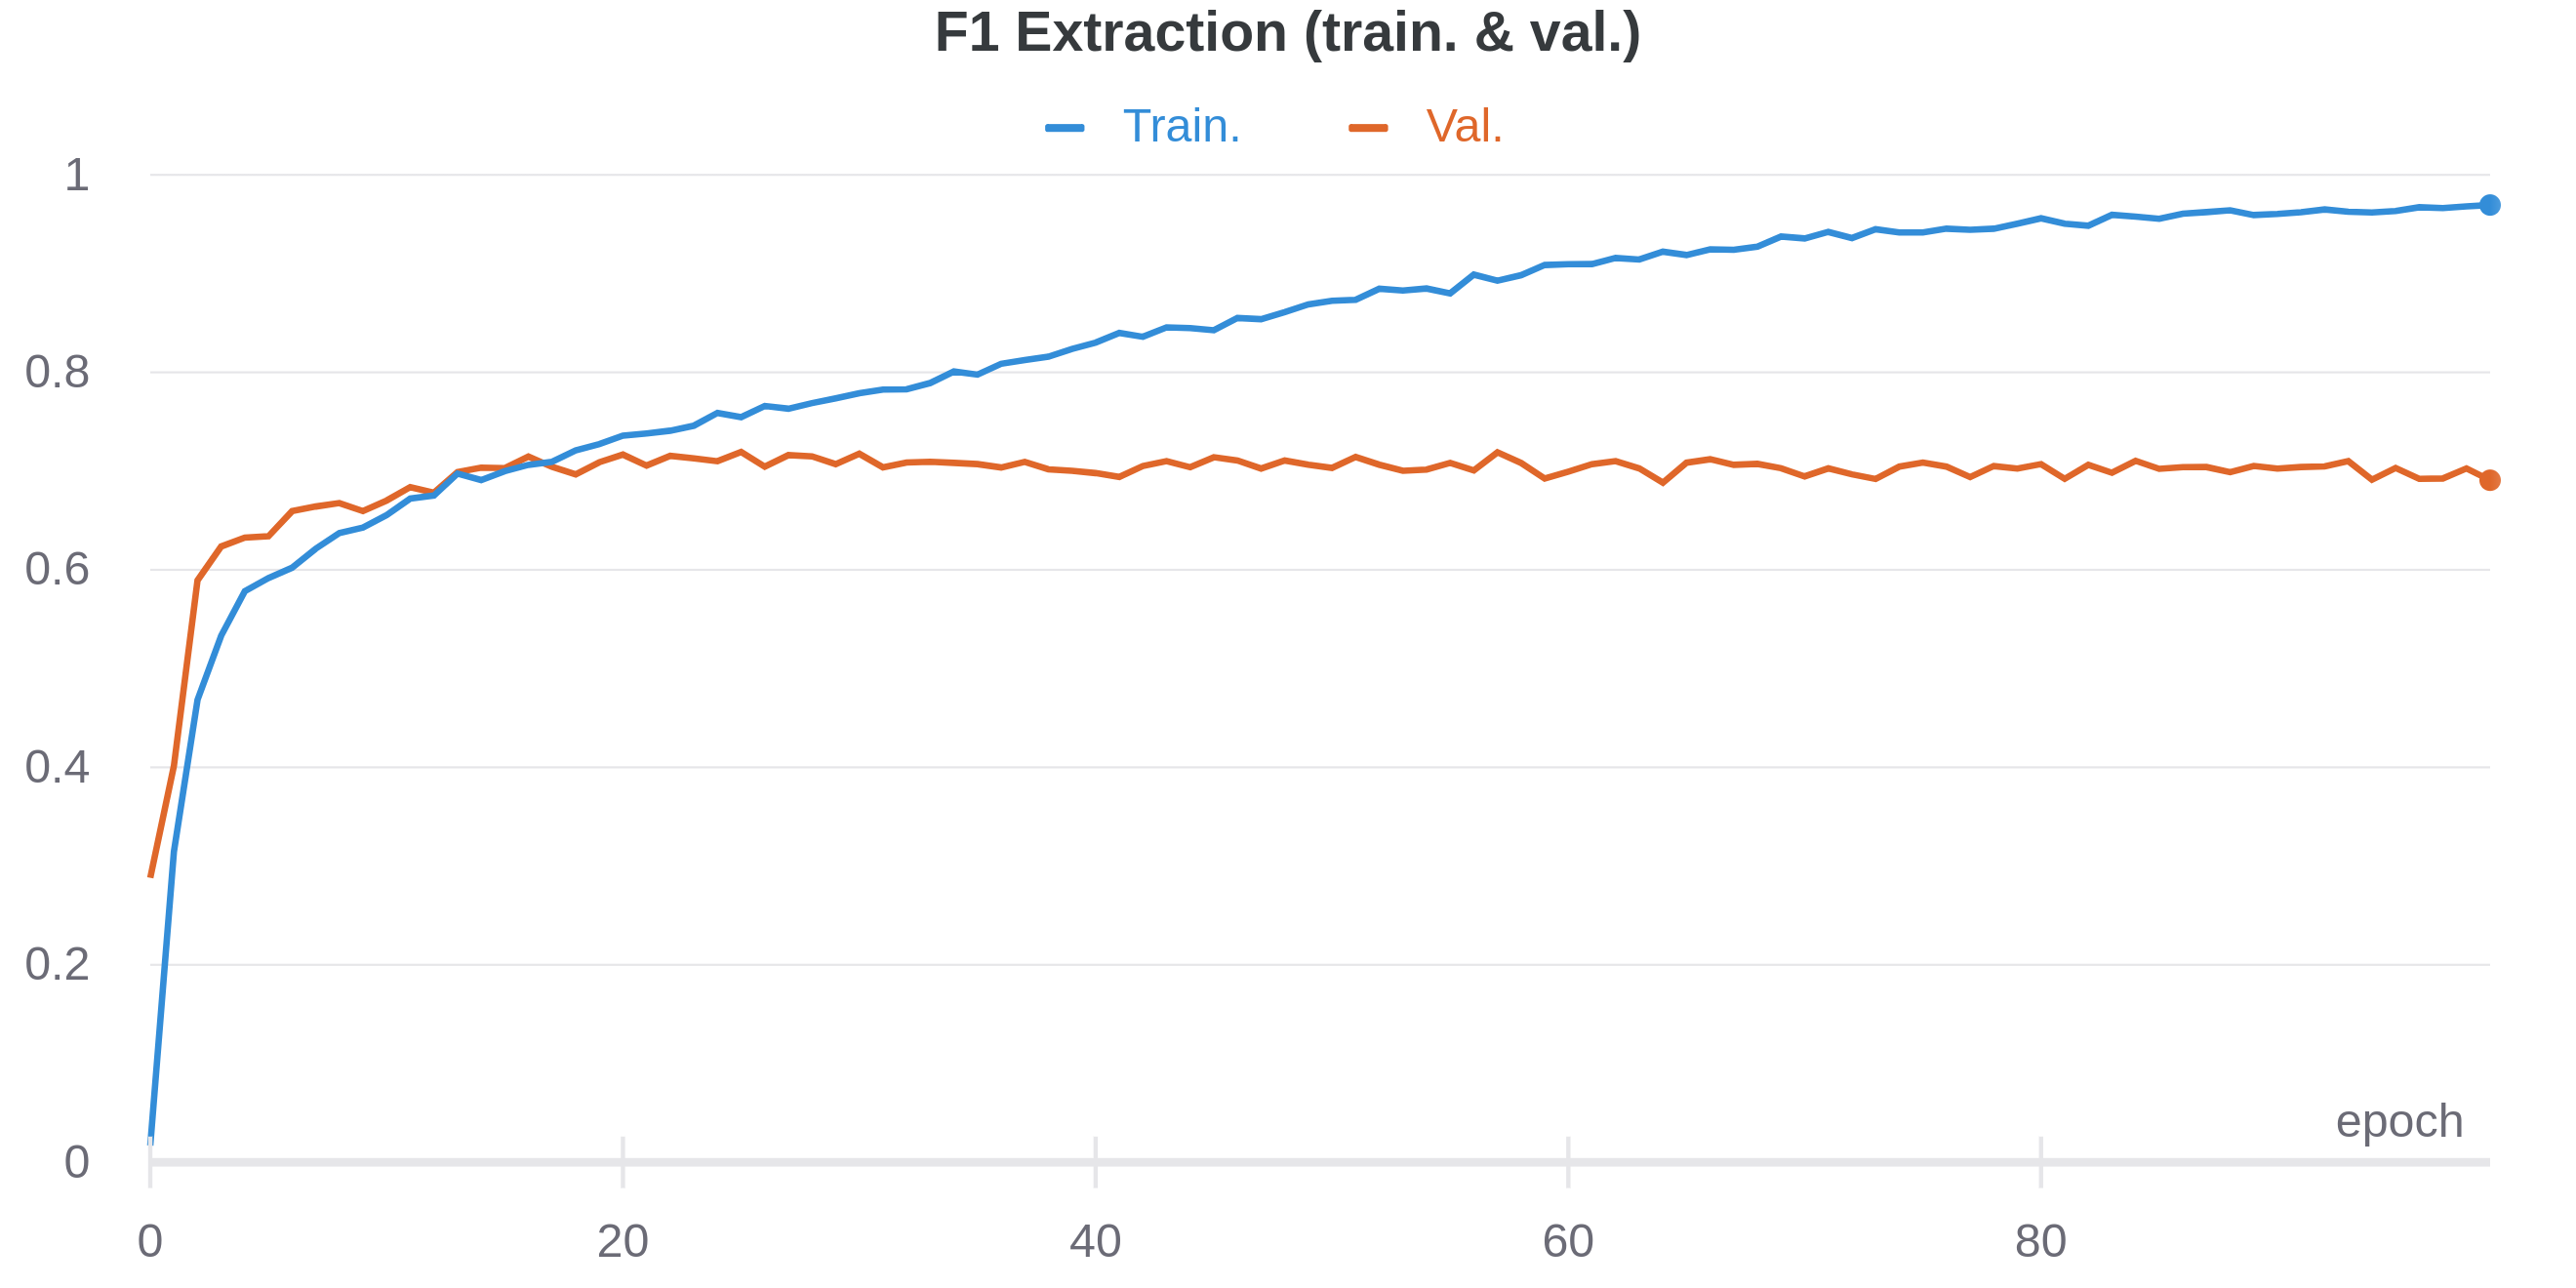
\includegraphics[width=1\columnwidth]{M0_ab_f1_extr.png}
		\caption{Task A+B: Baseline (M0) macro f1 extraction score on the training and
			development set.}
		\label{fig:M0_extr}
	\end{figure}
	
	\begin{figure}[H]
		\centering
		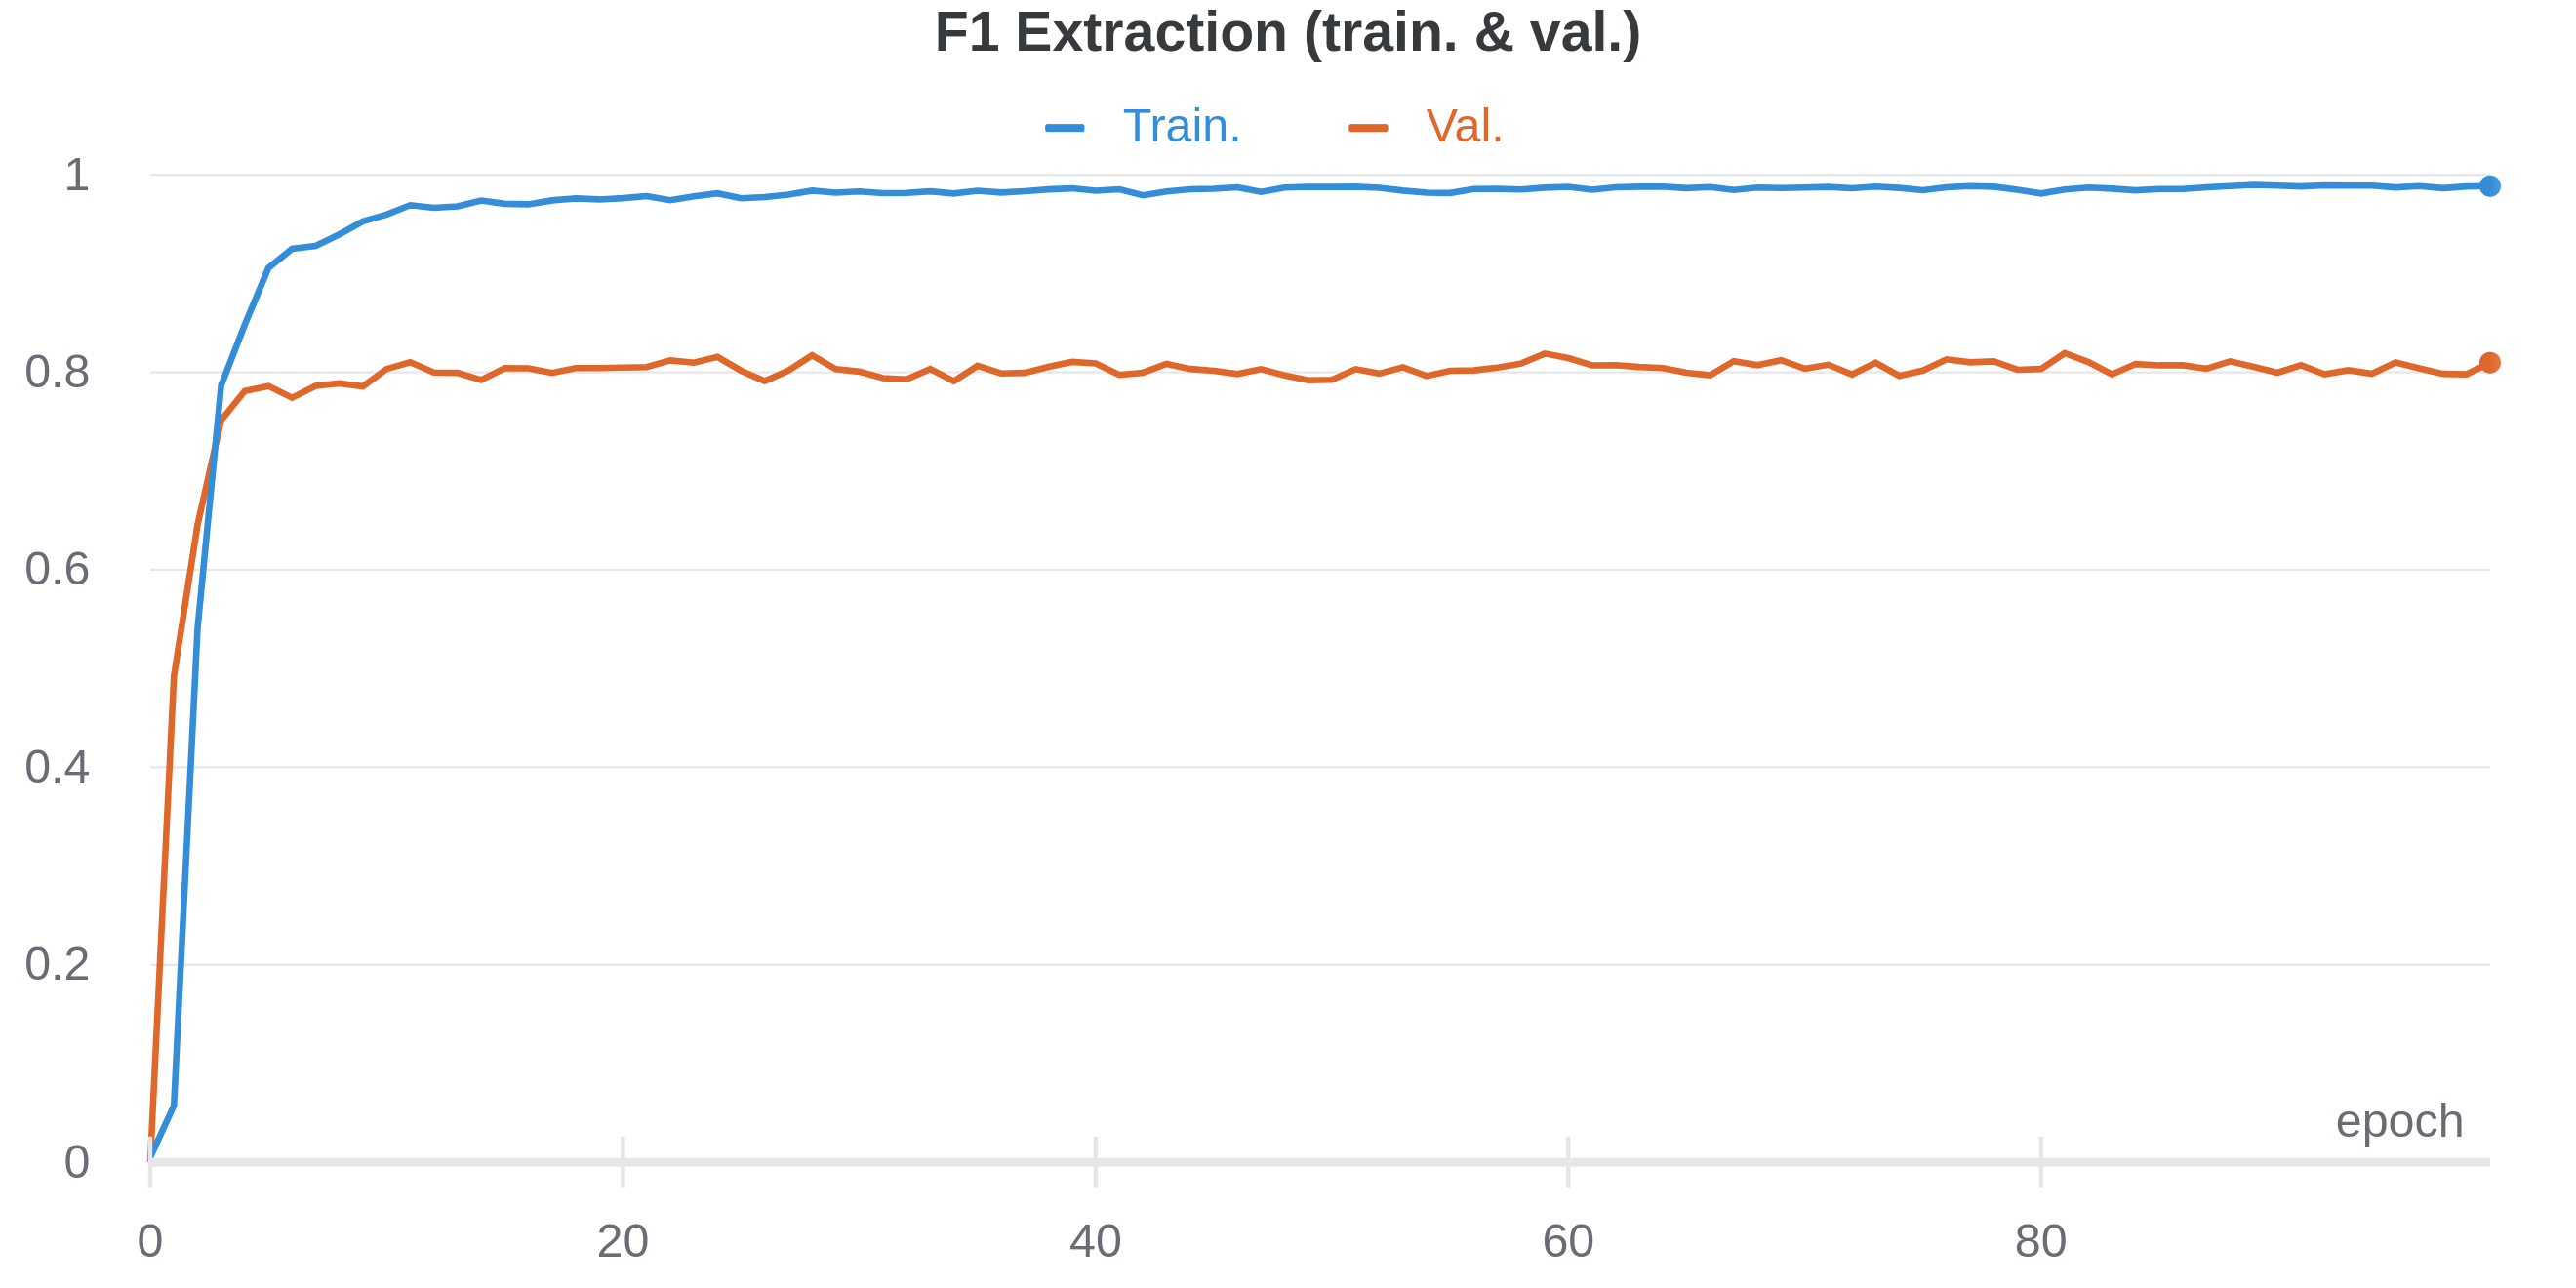
\includegraphics[width=1\columnwidth]{M3_ab_f1_extr.png}
		\caption{Task A+B: Final model (M3) macro f1 extraction score on the training
			and development set.}
		\label{fig:M3_extr}
	\end{figure}
	
	\begin{figure}[H]
		\centering
		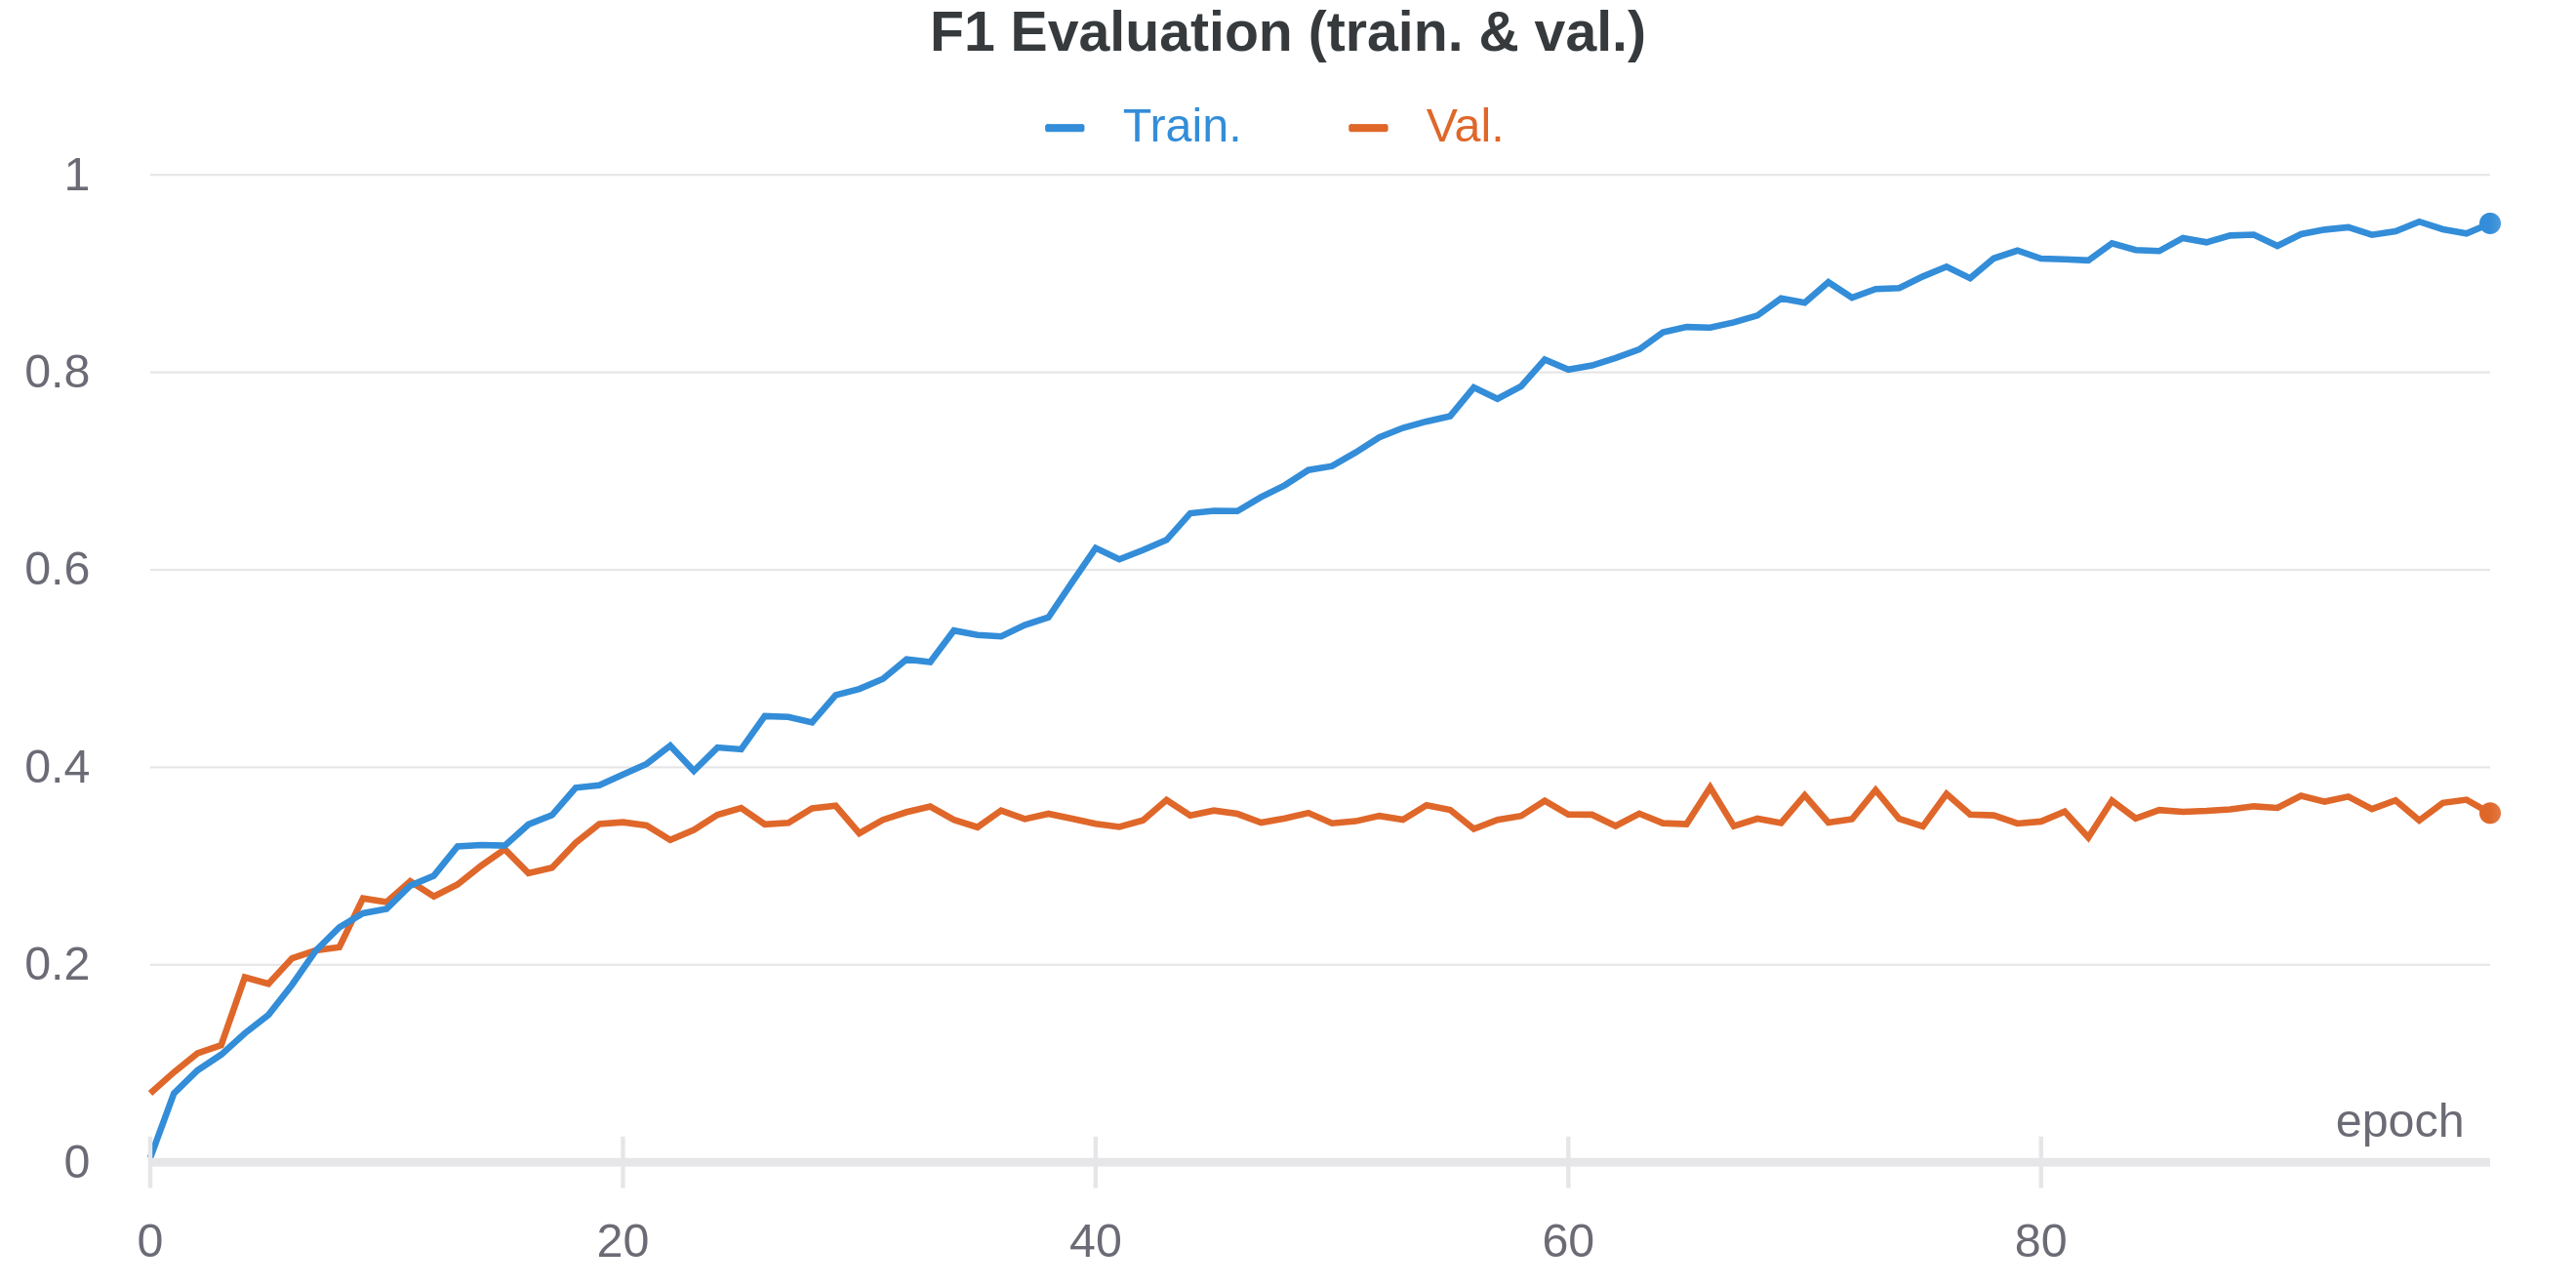
\includegraphics[width=1\columnwidth]{M0_ab_f1_eval.png}
		\caption{Task A+B: Baseline (M0) macro f1 evaluation score on the training and
			development set.}
		\label{fig:M0_eval}
	\end{figure}
	
	\begin{figure}[H]
		\centering
		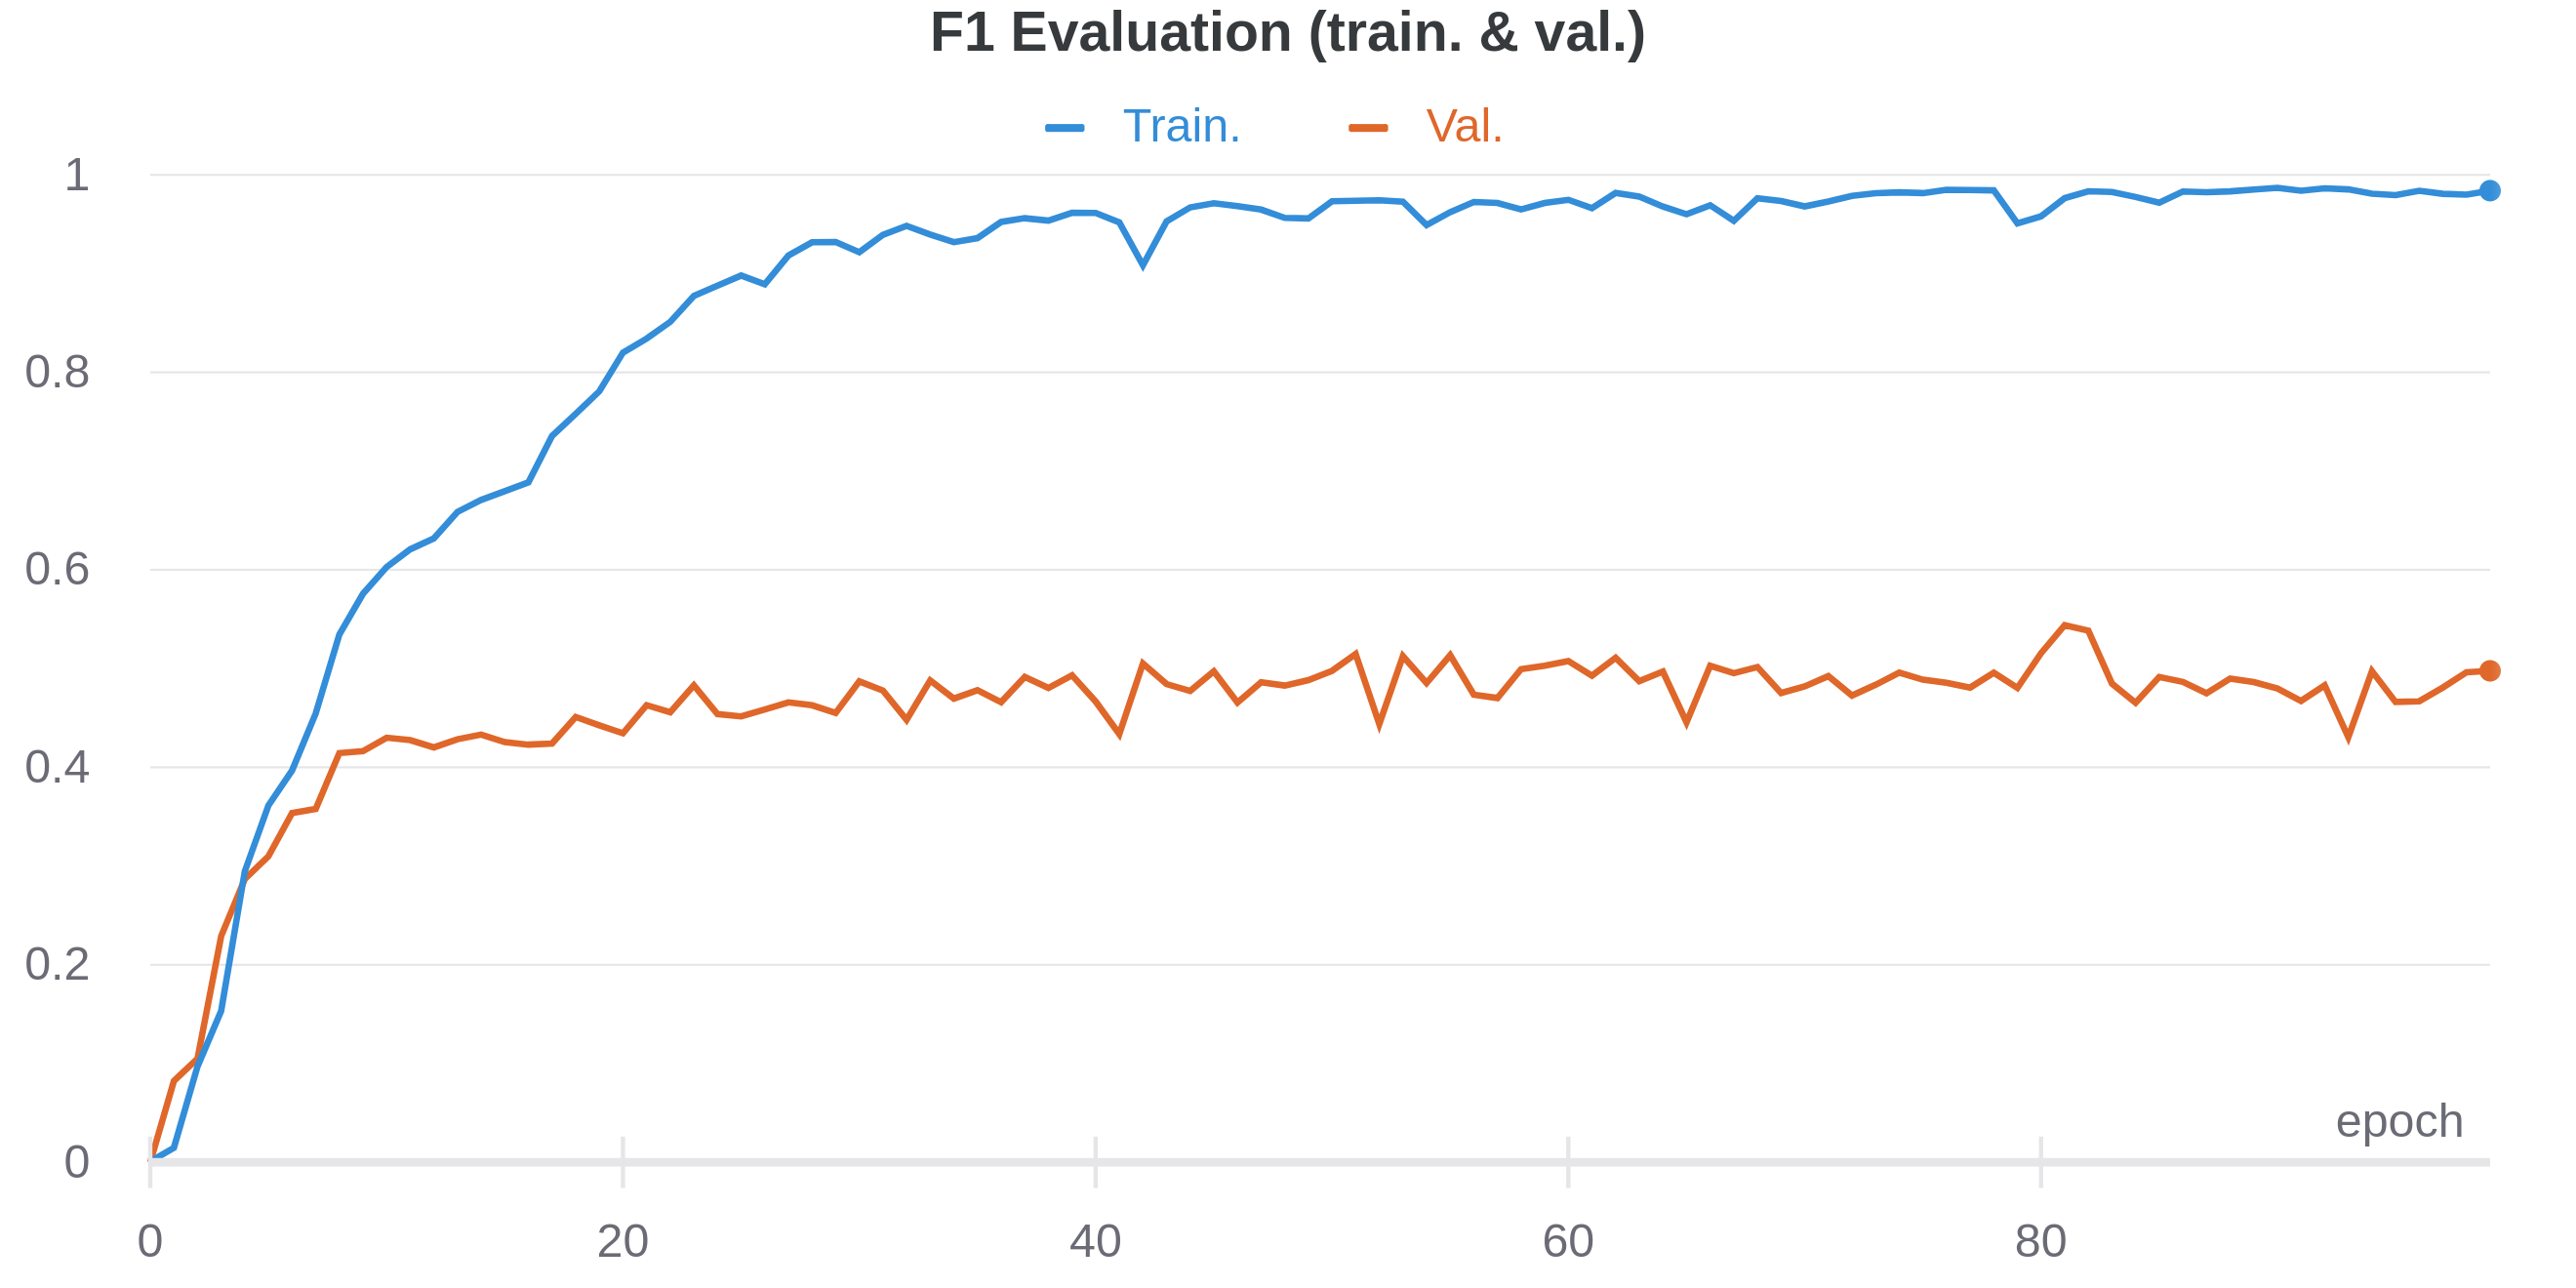
\includegraphics[width=1\columnwidth]{M3_ab_f1_eval.png}
		\caption{Task A+B: Final model (M3) macro f1 evaluation score on the training
			and development set.}
		\label{fig:M3_eval}
	\end{figure}
	
	\begin{figure}[H]
		\centering
		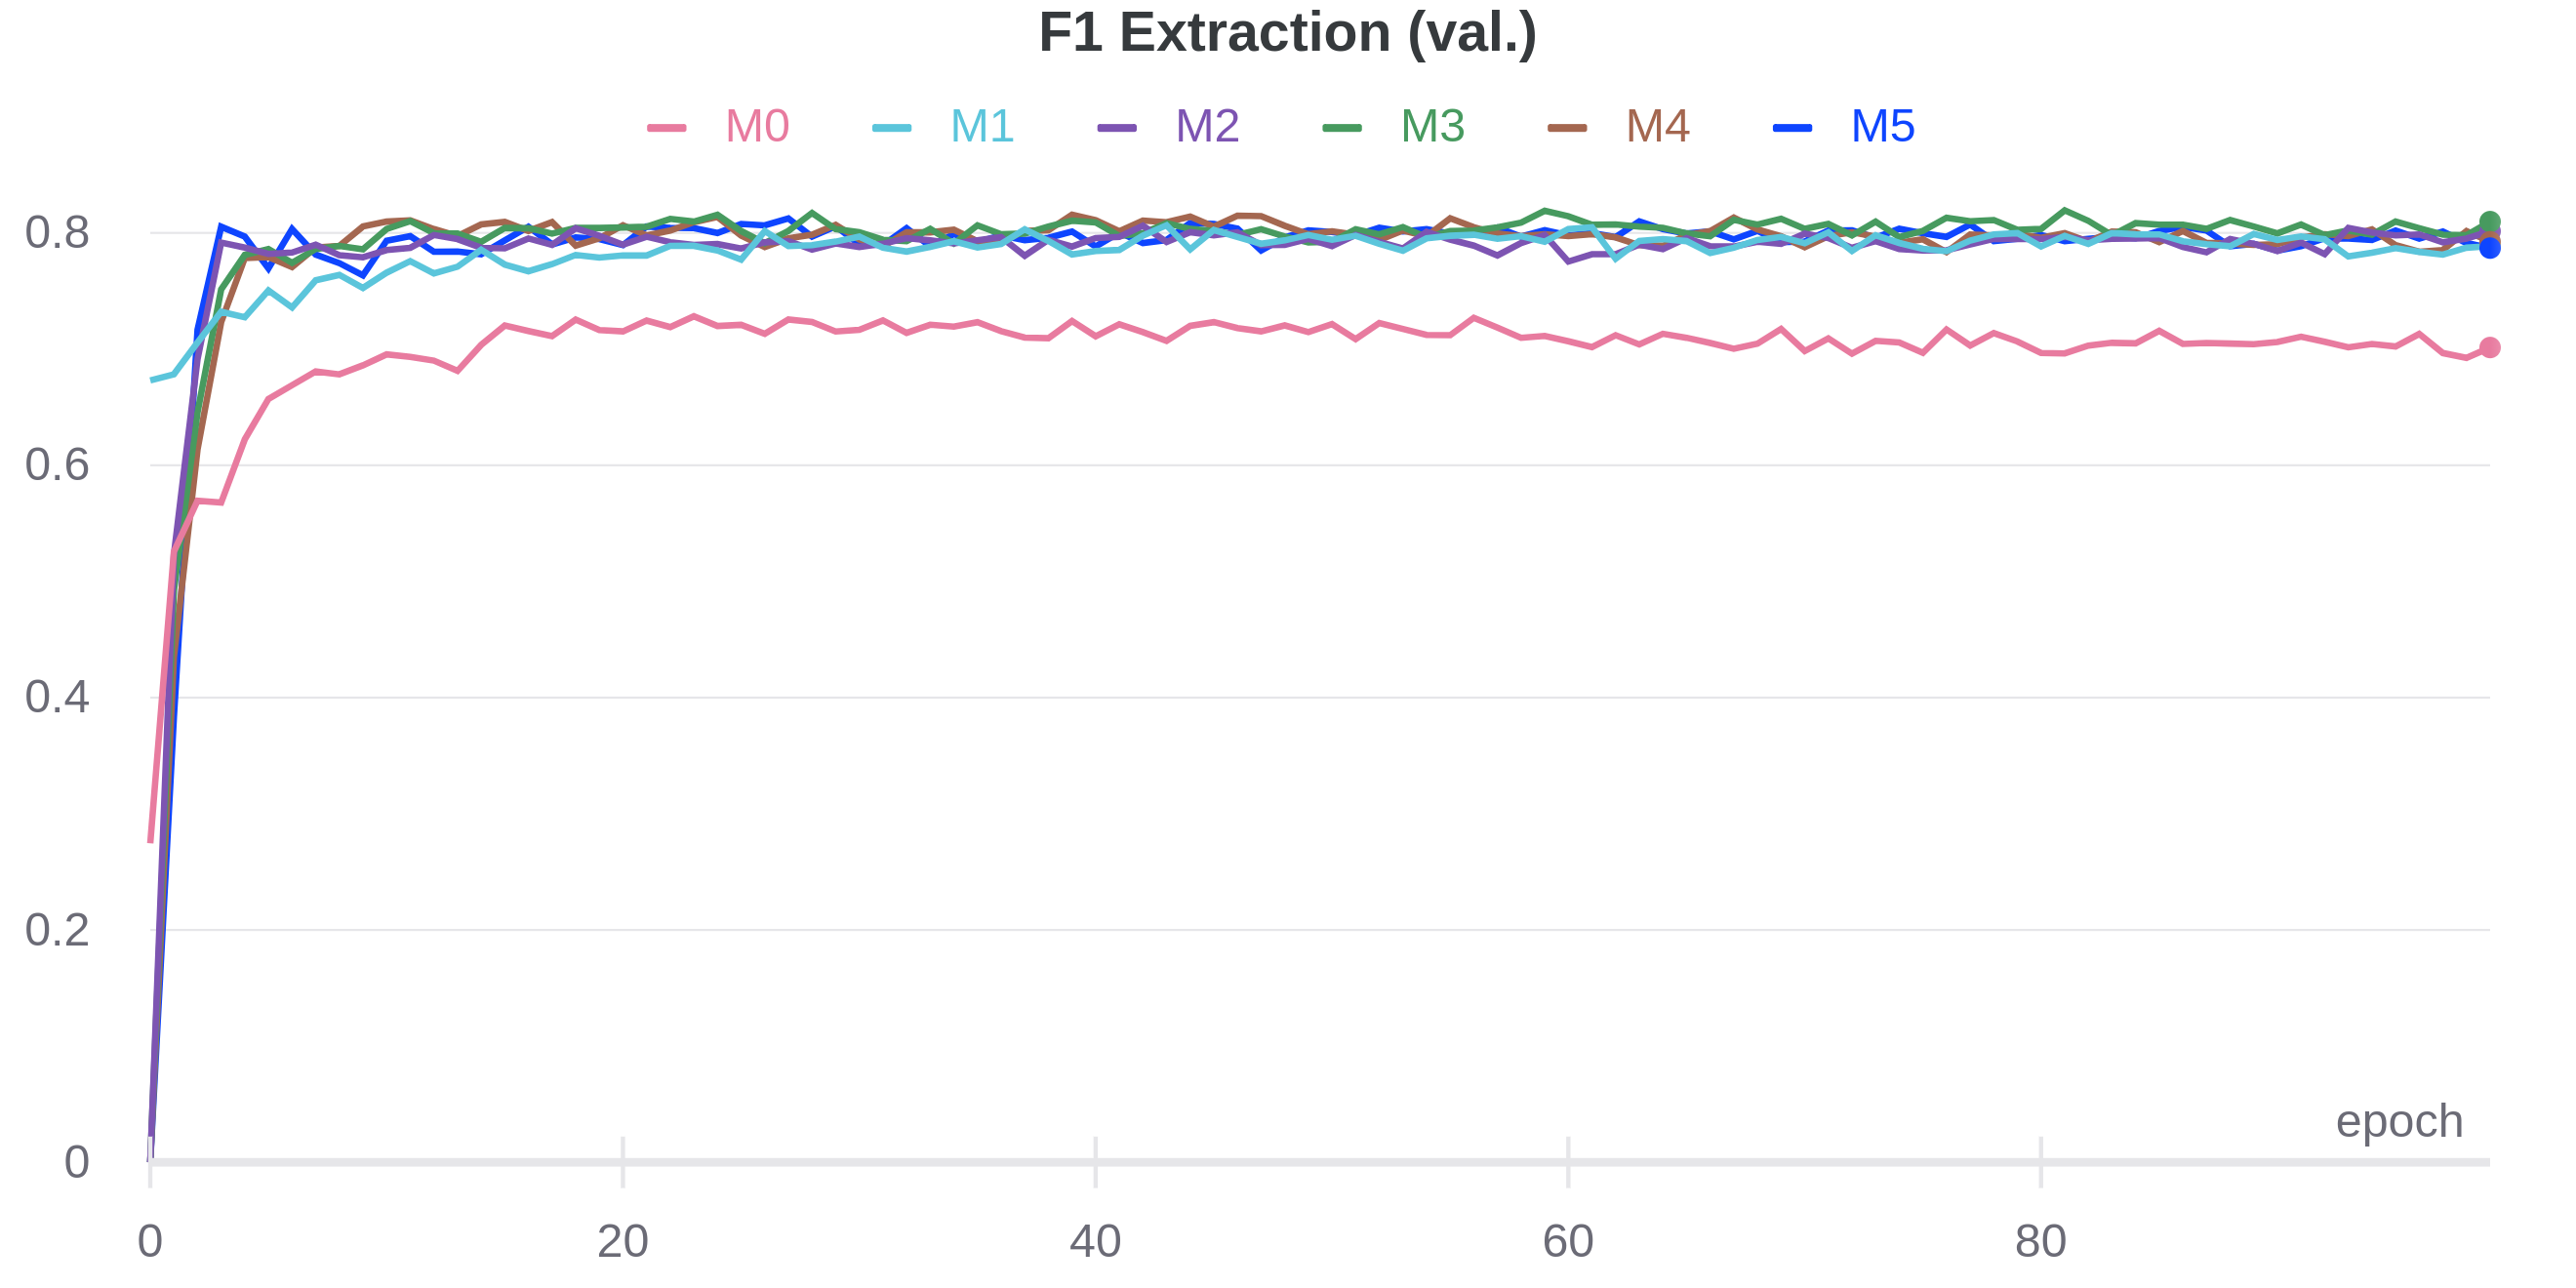
\includegraphics[width=1\columnwidth]{ab_comparative_f1_extr.png}
		\caption{Task A+B: Comparative plot of f1 extraction score for the 6 model
			variations (M0, M1, M2, M3, M4, M5).}
		\label{fig:comparative_f1_extr}
	\end{figure}
	
	\begin{figure}[H]
		\centering
		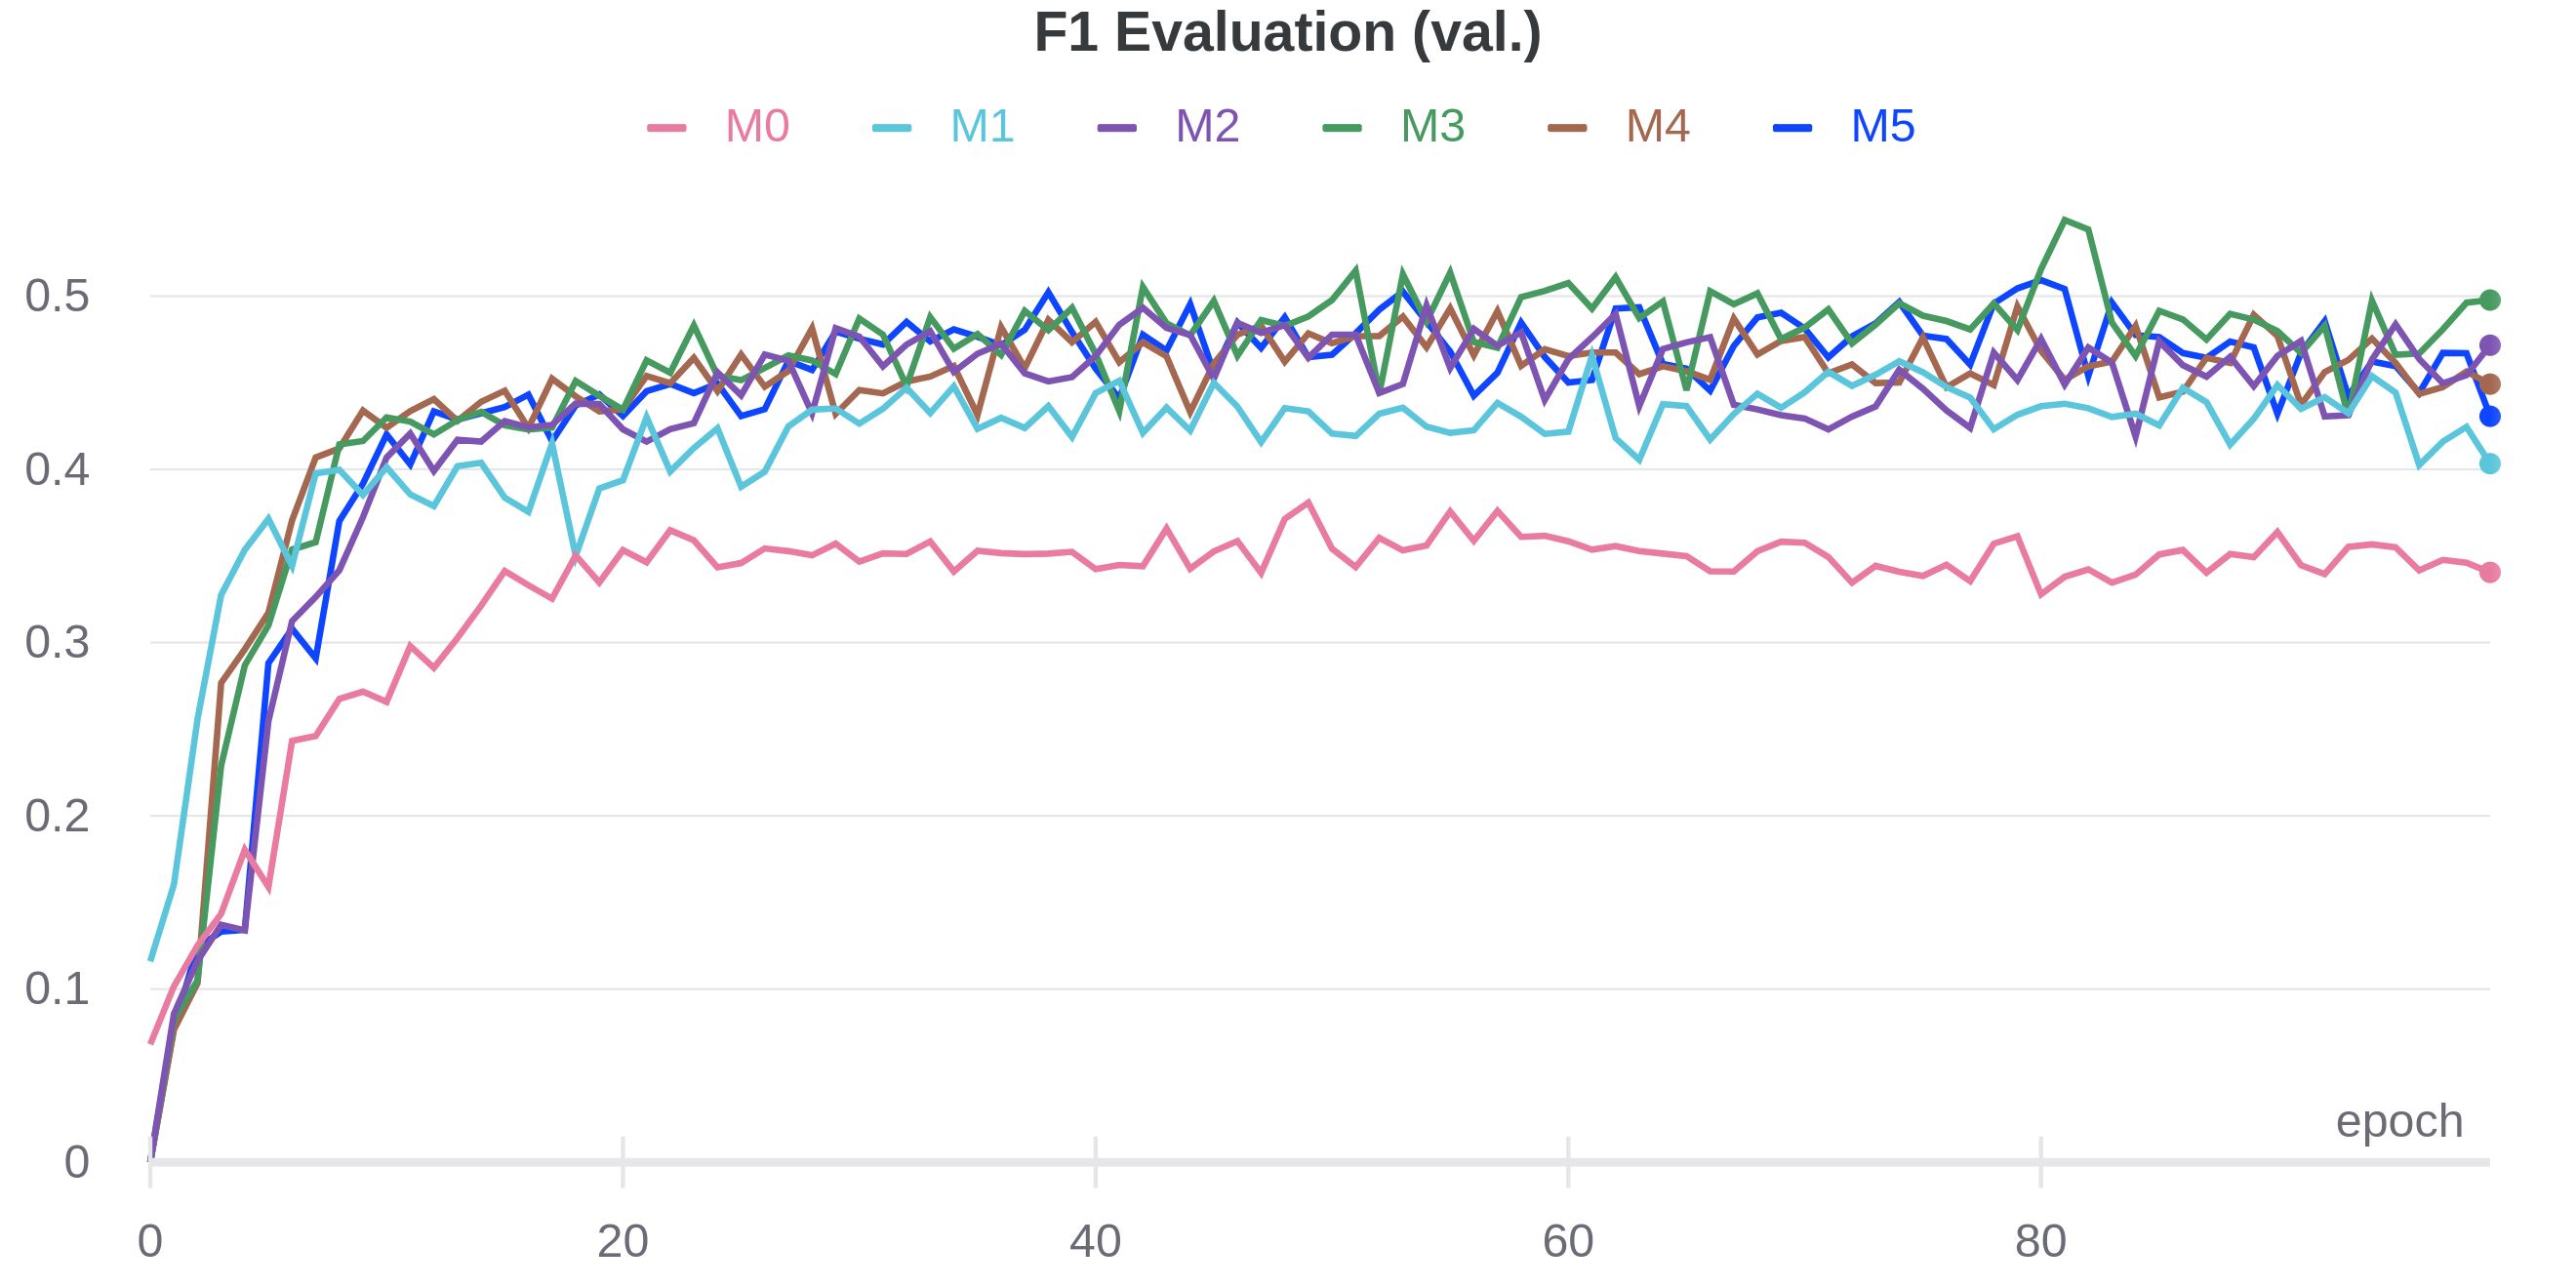
\includegraphics[width=1\columnwidth]{ab_comparative_f1_eval.png}
		\caption{Task A+B: Comparative plot of f1 evaluation score for the 6 model
			variations (M0, M1, M2, M3, M4, M5).}
		\label{fig:comparative_f1_eval}
	\end{figure}
	
	\begin{figure}[H]
		\centering
		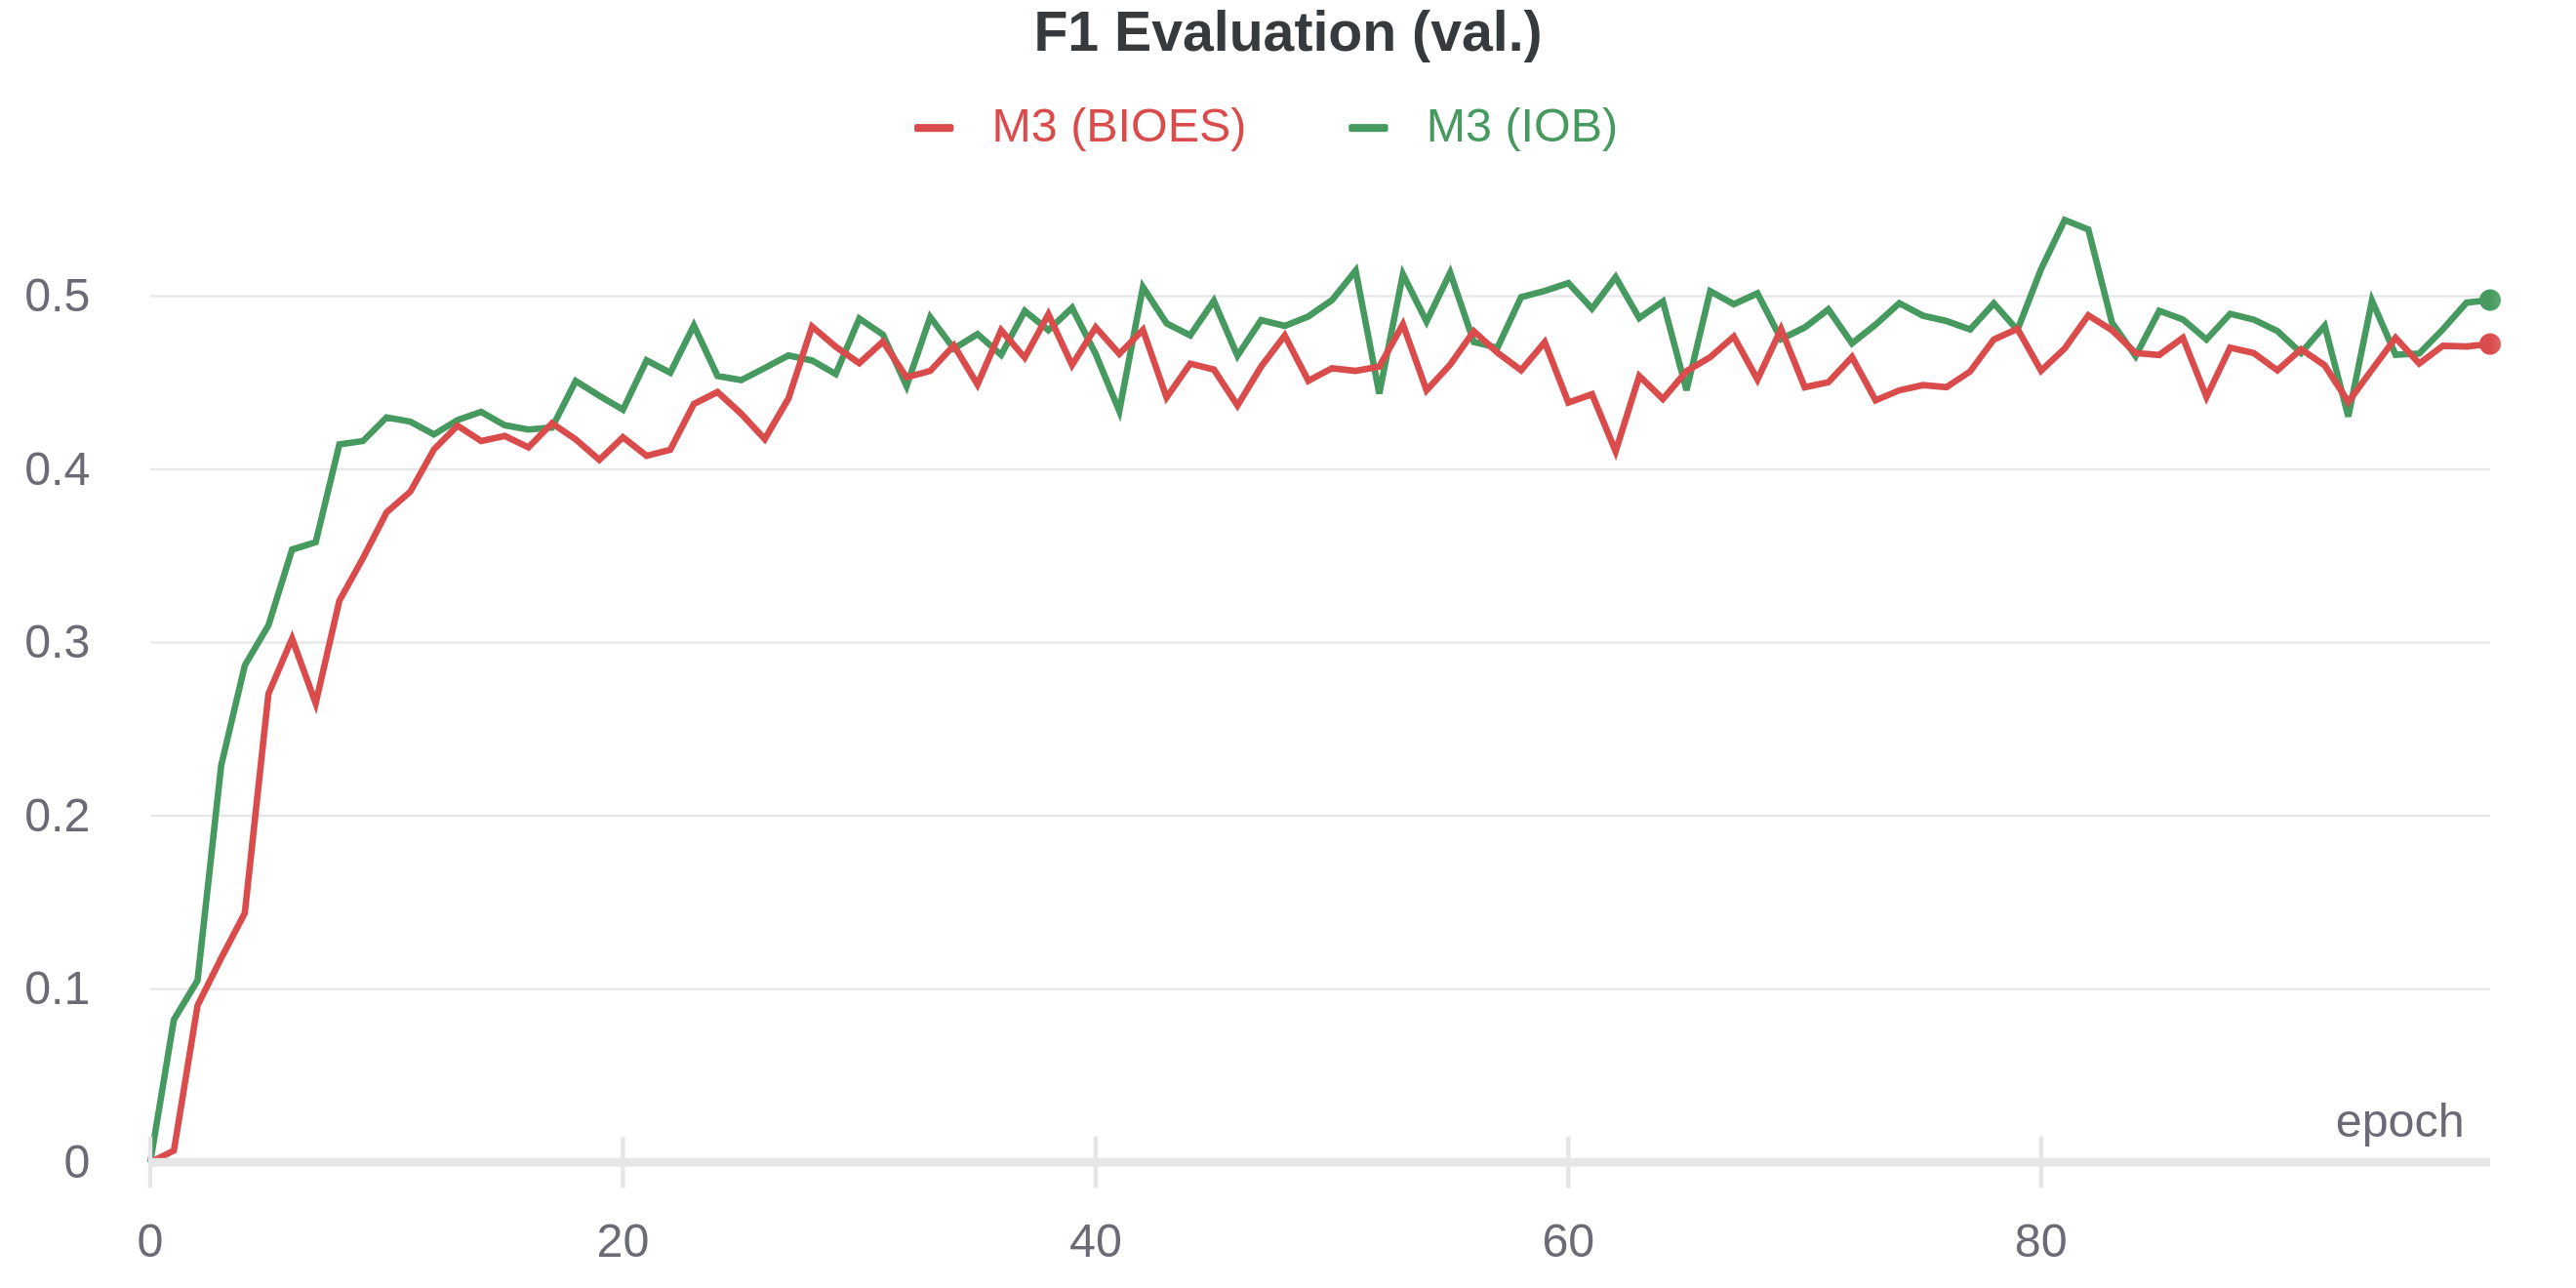
\includegraphics[width=1\columnwidth]{M3_ab_IOB_vs_BIOES_f1_extr.png}
		\caption{Task A+B: Comparative plot of f1 extraction score for the best model
			(M3) using two different tagging schemas (IOB, BIOES).}
		\label{fig:IOB_vs_BIOES_extr}
	\end{figure}
	
	\begin{figure}[H]
		\centering
		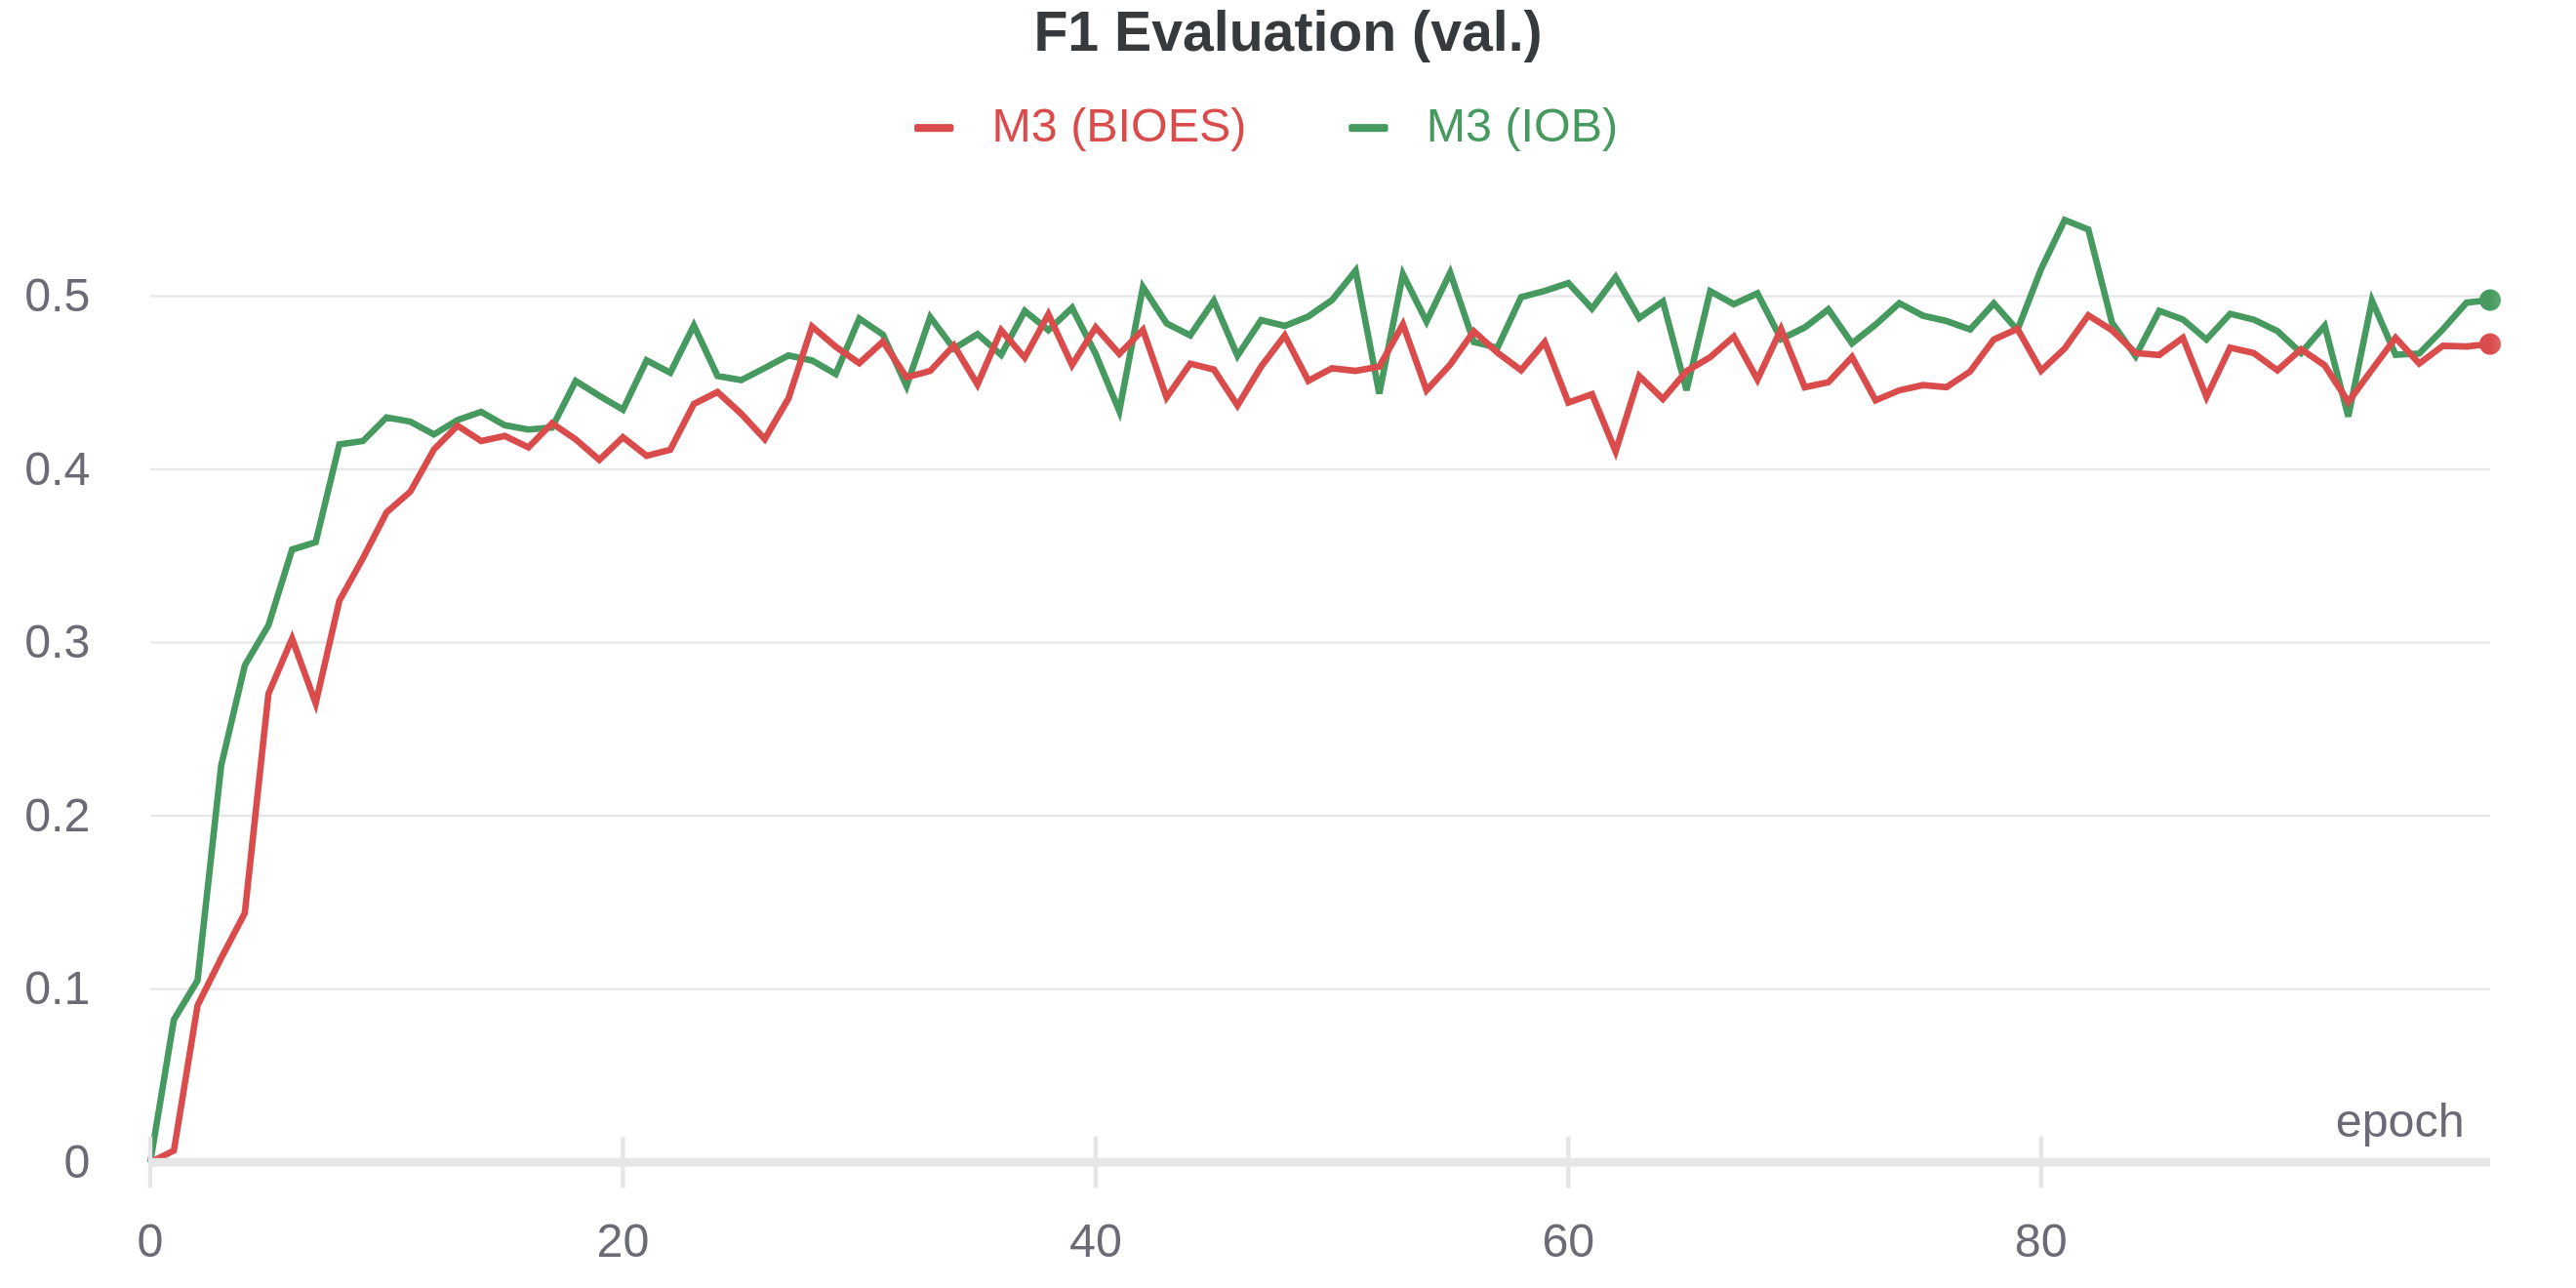
\includegraphics[width=1\columnwidth]{M3_ab_IOB_vs_BIOES_f1_eval.png}
		\caption{Task A+B: Comparative plot of f1 evaluation score for the best model
			(M3) using two different tagging schemas (IOB, BIOES).}
		\label{fig:IOB_vs_BIOES_eval}
	\end{figure}
	
	\begin{figure}[H]
		\centering
		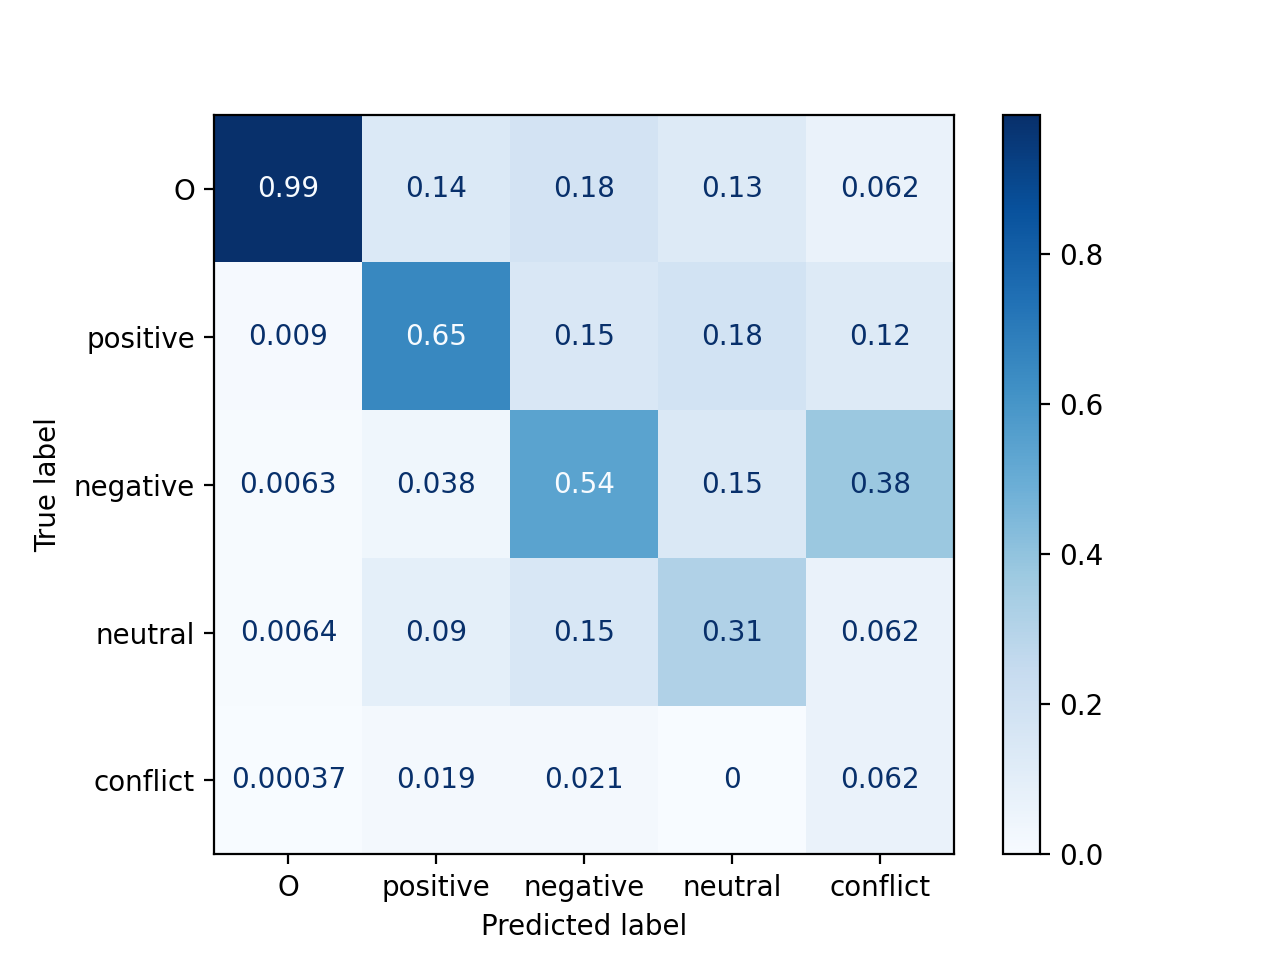
\includegraphics[width=1\columnwidth]{M0_ab_confusion_matrix.png}
		\caption{Task A+B: Normalized confusion matrix of the baseline model (M0).}
		\label{fig:cm_M0}
	\end{figure}
	
	\begin{figure}[H]
		\centering
		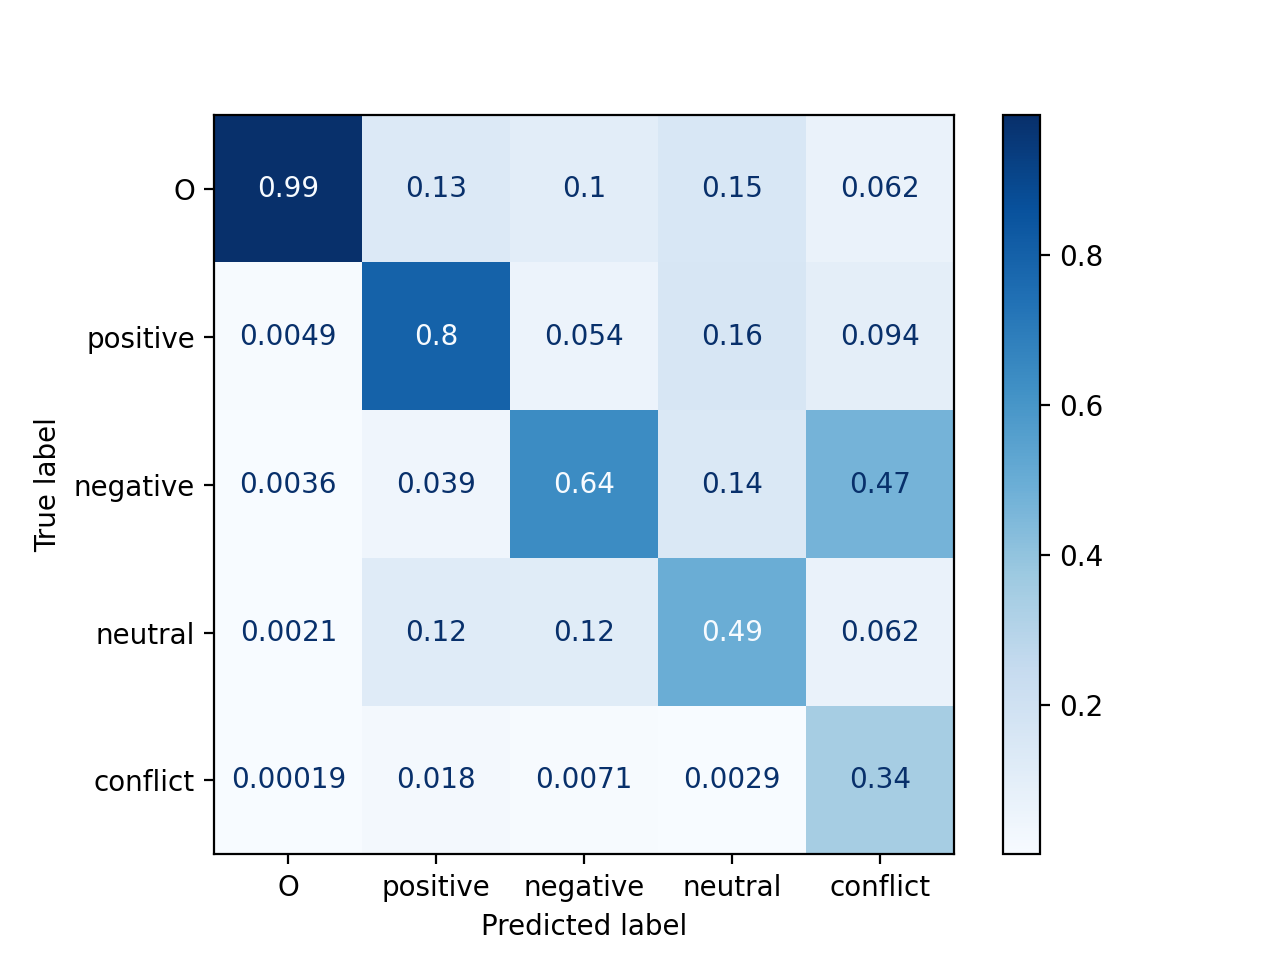
\includegraphics[width=1\columnwidth]{M3_ab_confusion_matrix.png}
		\caption{Task A+B: Normalized confusion matrix of the best model (M3).}
		\label{fig:cm_M3}
	\end{figure}
	
	\bibliographystyle{acl_natbib}
	\bibliography{bibliography}
	
	%\appendix
	
	
	
\end{document}
